%%%%%%%%%%%%%%%%%%%%%%%%%%%% %
% CH4 : Viscous flows : Laminar and turbulent flows %
%%%%%%%%%%%%%%%%%%%%%%%%%%%% %

\chapter{Viscous flows : Laminar and turbulent flows}
	\section{Illustrative example : channel flow}
		
		\begin{wrapfigure}[8]{l}{6.5cm}
		\vspace{-5mm}
		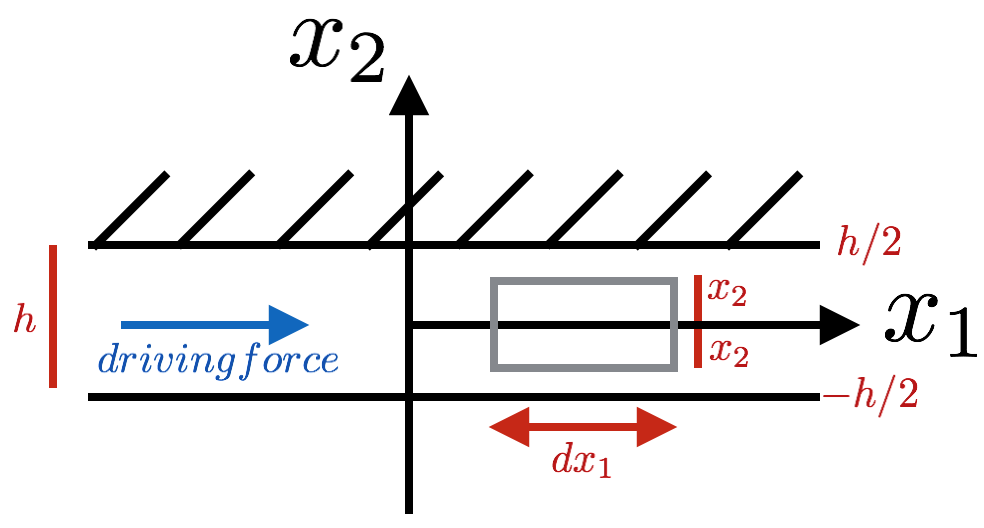
\includegraphics[scale=0.35]{ch4/1}
		\captionof{figure}{}
		\end{wrapfigure}
		It's the flow between two infinite parallel plates whiwh is driven by either a body force or a pression gradient. We will see that they can be linked together. We make the assumption that the flow is a \textbf{constant density flow} and \textbf{steady}. To analyse this, we need to choose a coordinates system. 

		\paragraph{Coordinates system}		
		We take $x_1$ in the direction of the driving force ($\rightarrow$) and $x_2$ normal to the plates, with the origin at the middel of the two plates. This is a planar flow, so
		\begin{equation}
			\Rightarrow  \frac{\D}{\D x_3}=0 \qquad and \qquad u_3 = 0 \mbox{ assumption}. 
		\end{equation}
		
		Because of the infinite plates, the origin can be everywhere on $x_1$ axis and the solution may not depend on it 
		\begin{equation}
			\frac{\D}{\D x_1} = 0 \qquad \mbox{(fully developed flow)}.
		\end{equation}
		This would not be the case if we had an entrance because the region near the entrance is not fully developed, we can see it as a transitory. Now let's make a momentum balance in a small region on $x_1$.
		
		\paragraph{$\mathbf{x_1}$ momentum balance}
			The time rate of change of the momentum inside a control volume + the net momentum flux going out is equal to 0 because there is no rate of change (steady) and the flow out is equal to the flow in (fully developed) 
			\begin{equation}
				0 = \mbox{sum of forces in } x_1.
			\end{equation}			 
		
		\paragraph{Mass balance} 
		It is the mass flow time rate of change + the mass out - mass in, the second and third term beeing null because velocity is constant
		\begin{equation}
			0 + \underbrace{\rho u_12x_2 |_{x_1+dx_1}- \rho u_12x_2 |_{x_1} }_{= 0} + \underbrace{\rho u_2 (x_1,x_2) -\rho u_2 (x_1,-x_2)}_{= 0} = 0.
		\end{equation}
		The third term teaches us that $2 \rho u_2(x_2)= 0 \Rightarrow u_2(x_2) = 0$. The other way to see that is to take the other form of the mass balance 
		\begin{equation}
			\cancel{\frac{\D\rho u_1}{\D x_1}}+\frac{\D\rho u_2}{\D x_2} = 0\qquad \Rightarrow \rho u_2 = cst = 0 \mbox{ (wall condition)}. 
		\end{equation}
		
		\begin{wrapfigure}[7]{l}{5.5cm}
		\vspace{-15mm}
		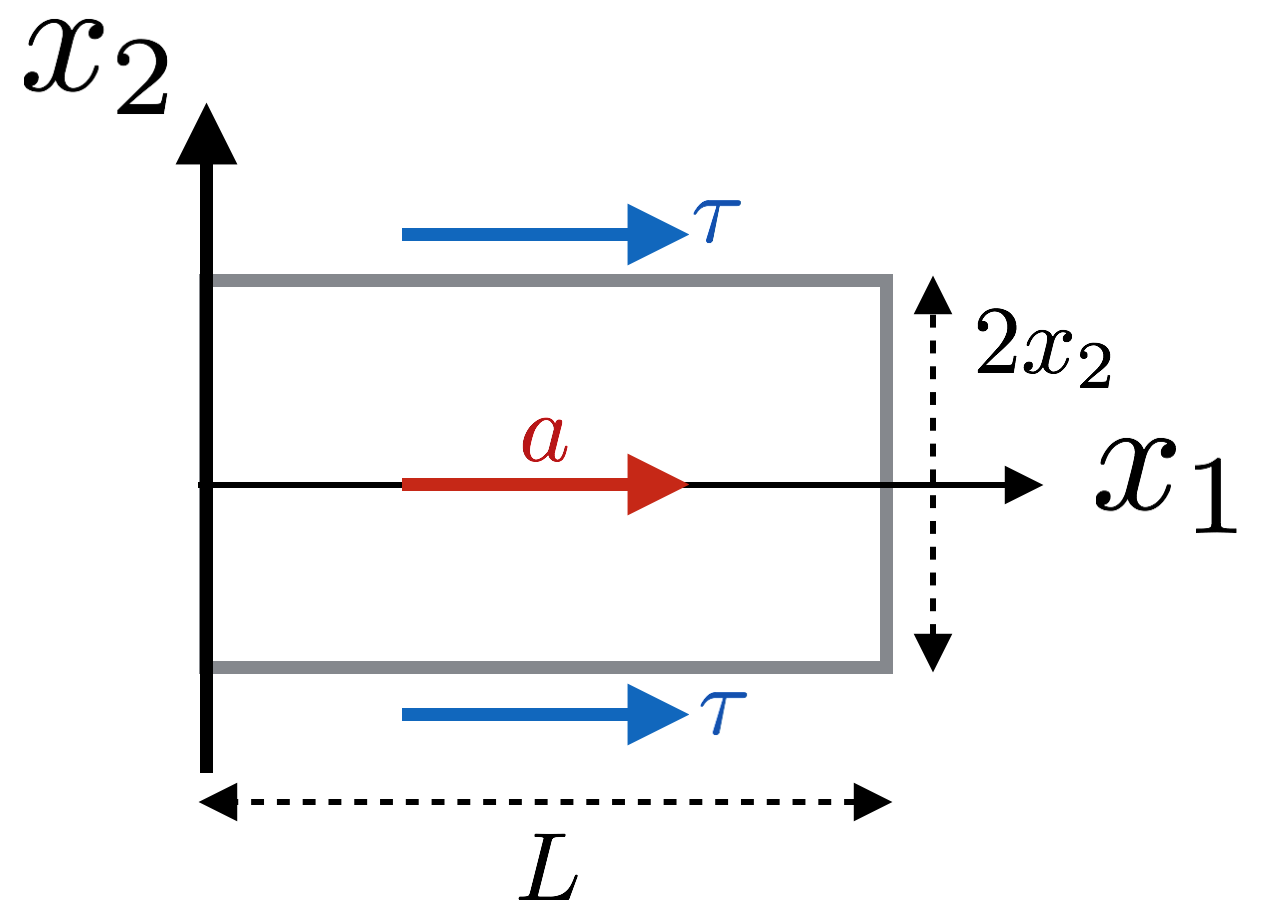
\includegraphics[scale=0.25]{ch4/2}
		\captionof{figure}{}
		\end{wrapfigure}
		\paragraph{Forces} There is the body force of acceleration $a \Rightarrow f_1 = am = a 2x_2 L \rho$, the pressure gradient $f_2 = (p_(0)-p(L))2x_2$ and the shear stress on the walls $f_3 = 2\tau L$, so
		\begin{equation}
		\begin{aligned}
			(p(0)-p(L))2x_2 +  a 2x_2 L \rho + 2\tau L = 0 \\
			\Rightarrow \tau = -x_2 \left( \rho a - \frac{p(L)-p(0)}{L}\right) = -x_2 f_1
		\end{aligned}
		\end{equation}
		\ \\
			
		\begin{wrapfigure}[7]{r}{5cm}
		\vspace{-15mm}
		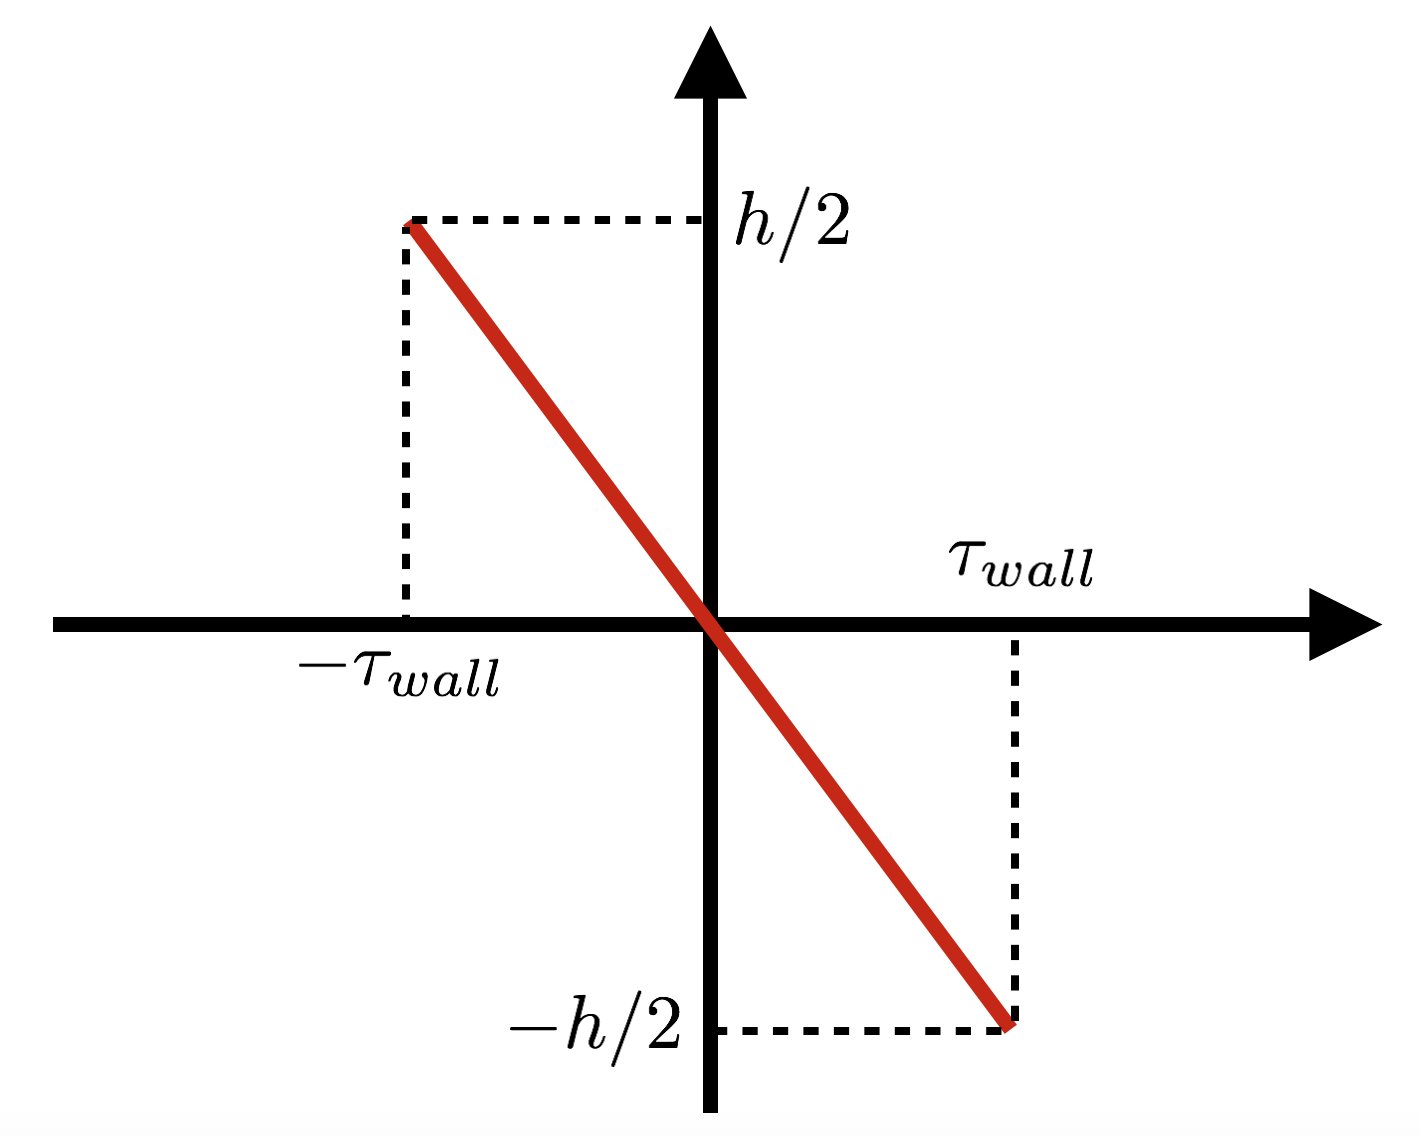
\includegraphics[scale=0.2]{ch4/3}
		\captionof{figure}{}
		\label{fig:4.3}
		\end{wrapfigure}
		where $f_1 = \rho a - \frac{dp}{dx} = -\frac{d\hat{p}}{dx}$ is the driving force (force per unit volume) and $\hat{p} = p - \rho a$ the driving pressure, we see that even the pressure gradient appears in his expression. The evolution of the linear $\tau$ is represented on \autoref{fig:4.3}, shear stress representing the effect of the upper part on the lower part, it seems legit to have $-\tau$ for the upper wall meaning that the wall slows down the fluid (below the fluid drag the wall). The velocity profile can be found as 
		\begin{equation}
			\tau = -x_2 f_1 = \mu \left( \frac{\D u_1}{\D x_2}+ \cancel{\frac{\D u_2}{\D x_1}}\right) \qquad \Rightarrow \mu \frac{\D u_1}{\D x_2} = -x_2 f_1 \Leftrightarrow u_1 = \frac{f_1}{2\mu} (-x_2^2+cst).
		\end{equation}
		
		\begin{wrapfigure}[7]{r}{3.6cm}
		\vspace{-5mm}
		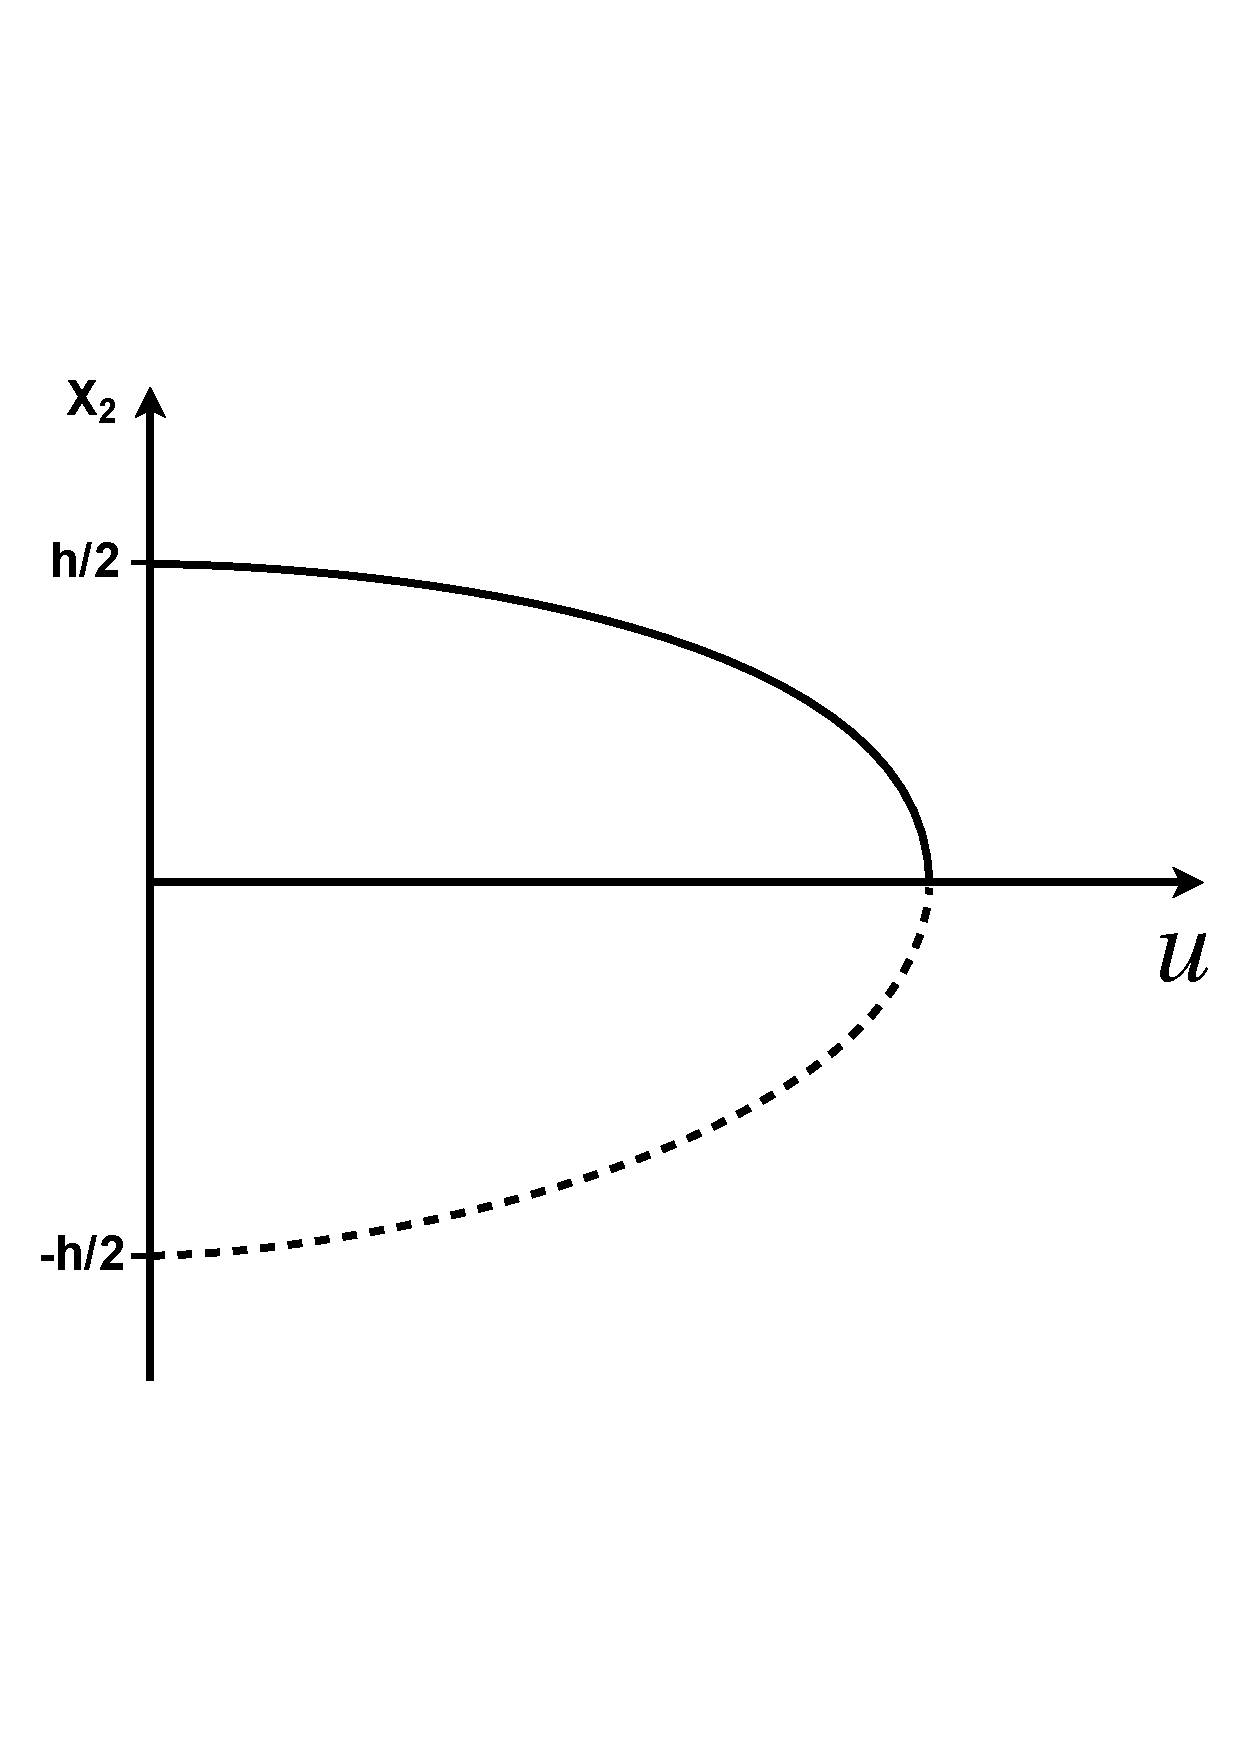
\includegraphics[scale=0.2]{ch4/4}
		\captionof{figure}{}
		\label{fig:4.4}
		\end{wrapfigure}
		The non slip boundary condition at the wall gives $u_1(\pm \frac{h}{2}) \Rightarrow c =\left( \frac{h}{2}\right)^2$. The velocity profile is 
		\begin{equation}
			u_1 = \frac{f_1}{2\mu} \left(\left(\frac{h}{2}\right)^2-x_2^2\right)
			\label{eq:4.8}
		\end{equation}
		which is parabolic as shown on \autoref{fig:4.4} with a maximum on $x_1$ axis of value $u_1 = \frac{f_1h^2}{8\mu}$. It is also interesting to compute the volume flow per unit span $[m^2/s]$ ($x_3$) 
		\begin{equation}
			\dot{V} = \int _{-h/2}^{h/2} u_1 \, dx_2 = \frac{2}{3} h \frac{f_1h^2}{8\mu} = \frac{f_1h^3}{12\mu} 
		\end{equation}
		where the integral has been computed using the definition of the era of the parabole $2/3 \times h \times u_c$. 
		
		\paragraph{Dimensional analysis}
		Imagine that we would have liked to determine the velocity profile by dimensional analysis. The veloity dependance is 
		\begin{equation}
			u_1 = f(x_2, f_1, h, \mu ,\rho )
		\end{equation}
		giving us 6 variables and 3 physical dimensions and so 3 dimensionless groups.   To make the velocity dimensionless, we computed the velocity at the center, let's use it. The dimensionless velocity will be function of 2 dimensionless groups 
		\begin{equation}
			\frac{u_1}{\frac{f_1h^2}{8\mu}} = \varphi \left( \frac{2x_2}{h}, Re = \frac{u_c h}{\nu} = \frac{\rho f_1 h^3}{8 \mu ^2} \right).			
		\end{equation}		 
		Now if we rewrite \eqref{eq:4.8} as 
		\begin{equation}
			u_1 = \frac{f_1h^2}{8\mu}\left( 1 - \left( \frac{2x_2}{h}\right) ^2\right).
		\end{equation}
		
	 	\begin{wrapfigure}[10]{l}{3.6cm}
		\vspace{-5mm}
		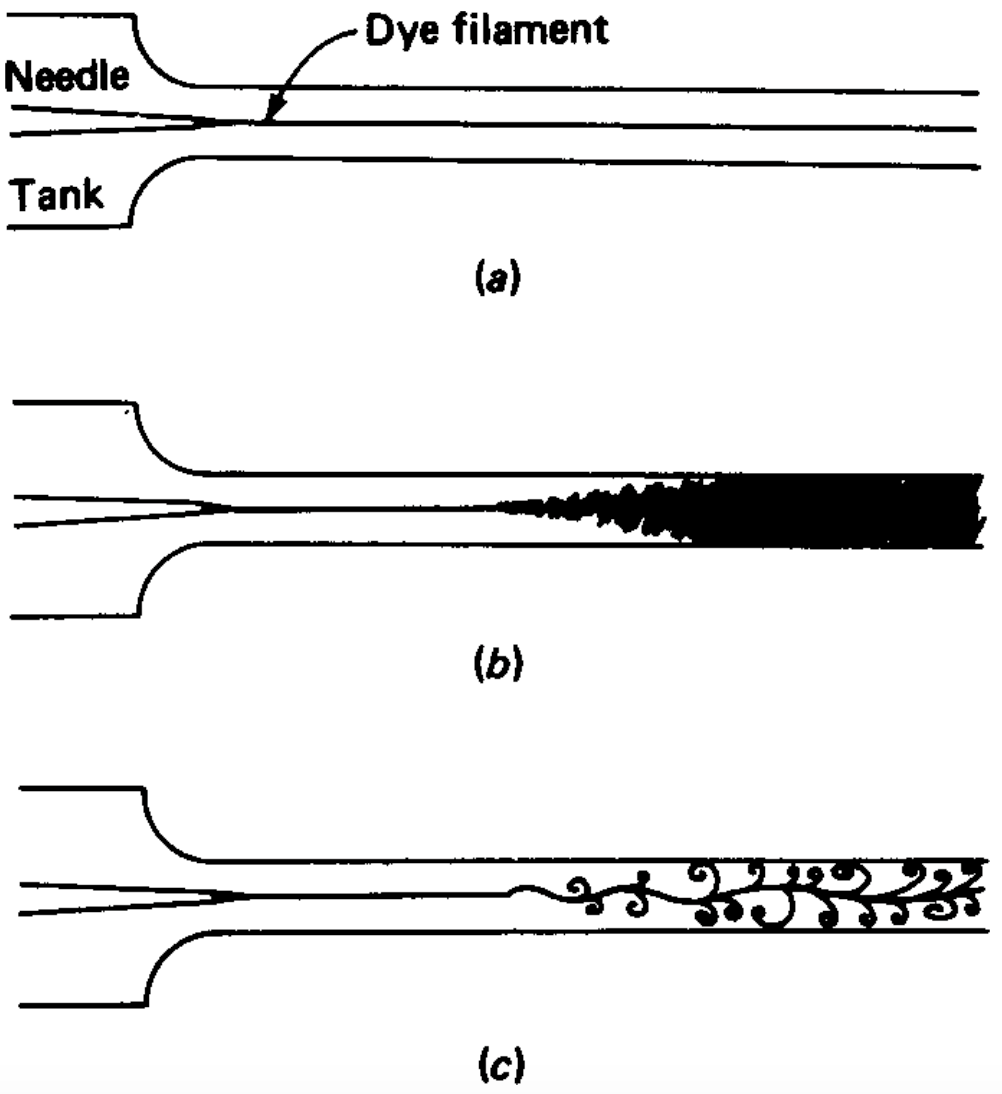
\includegraphics[scale=0.2]{ch4/5}
		\captionof{figure}{}
		\end{wrapfigure}
		When we compare the 2 equations, we see that $\varphi = f(x_2/h)$. That means that when we solve the equation there is no dependance on the Re number. So the dimensional analysis doesn't give the full information, we have to solve. Re number is the ratio between viscous forces and conventional inertial forces. Because of fully developed criteria there is no conventional inertial forces, it is normal so that the flow does not depend on the Re number. This parabolic profile is respected for low velocities but disturb when velocity increases. We made the assumption that the flow is steady, but for a certain velocity the flow is no longer steady, it becomes chaotic (turbulences). 
		

\section{Macroscopique des cription of turbulent flows - Reynolds decomposition}
	The interest of this approach is in the mean flow, in average quantities. The idea is to repeat the experiment several times and make a statistical average in order to decompose all variables into an average and a fluctuation. This is called the Reynolds decomposition
	\begin{equation}
	\begin{array}{c}
		\forall \ quantity \ q : \langle q(x_1,x_2,x_3,t)\rangle =  \frac{1}{N} \sum _{k=1}^N q_k(x_1,x_2,x_3,t)\\ \\
		and \\ \\
		q_k(x_1,x_2,x_3,t) = \underbrace{\langle q_k(\cdots )\rangle}_{average} + \underbrace{q_k(\cdots )}_{fluctuation}
	\end{array}
	\end{equation}
	where $k$ is the experiment index. We are going to derive equations for the average properties for statistically steady flows (such that $\frac{\D \langle q\rangle}{\D t} = 0$). We can consider the time average with a certain period $T$
	\begin{equation}
		\bar{q}_T (x_1,x_2,x_3,t) = \frac{1}{T} \int _{t-T/2}^{t+T/2} q(x_1,x_2,x_3,t) \, dt
	\end{equation}
	which "smooth" the signal by keeping only large time scale fluctuations. For statistically steady flows, the \textbf{ergodicity hypothesis} is valid 
	\begin{equation}
		\lim _{T\rightarrow \infty} \bar{q}_T =  \langle q \rangle .
	\end{equation}
	For statistically unsteady flows, it is valid only if $T$ is much larger than the turbulent fluctuations time scale and much smaller than the average motion time scale. 
	
	\subsubsection{Properties of the averaging operator}

\begin{itemize}
\item[•] \textbf{Linearity :}
\begin{equation}
\langle a q_1 + bq_2\rangle = a \langle q_1\rangle + b  \langle q_2 \rangle 
\end{equation}

\item[•]
\begin{equation}
\langle \langle q\rangle \rangle = \langle q \rangle 
\end{equation}

\item[•]
\begin{equation}
\langle q'\rangle  = 0 \qquad as \qquad \langle q \rangle = \langle \langle q\rangle  + q'\rangle = \langle \langle q \rangle \rangle + \langle q'\rangle  =  \langle q\rangle  + \langle q'\rangle  \Rightarrow \langle q'\rangle  = 0
\end{equation}

\item[•]
\begin{equation}
\langle\langle q_1\rangle q_2\rangle = \langle q_1 \rangle \langle q_2\rangle
\end{equation}

\item[•] \textbf{Commutativity with differential operators}
\begin{equation}
	\left\langle \frac{\D q}{\D x_1} \right\rangle = \frac{\D \langle q \rangle}{\D x_1} \qquad \left\langle \frac{\D q}{\D t} \right\rangle = \frac{\D \langle q \rangle}{\D t}
\end{equation}
\end{itemize}

\subsubsection{Average continuity equation}
	Let's remind that we are considering \textbf{constant density} flow. In this case the governing equation for mass is
	\begin{equation}
		\cancel{\dot{\rho}} + \rho \nabla \vec{u} = 0 \qquad \Rightarrow \nabla \vec{u} = 0 = \frac{\D u_i}{\D x_i}
	\end{equation}
	Let's average this out 
	\begin{equation}
		\left\langle \frac{\D u_i}{\D x_i}  \right\rangle = \left\langle \frac{\D u_1}{\D x_1} + \frac{\D u_2}{\D x_2} + \frac{\D u_3}{\D x_3} \right\rangle = 		\left\langle \frac{\D u_1}{\D x_1}  \right\rangle  + \left\langle \frac{\D u_2}{\D x_2}  \right\rangle  + 	\left\langle \frac{\D u_3}{\D x_3}  \right\rangle  = 0
	\end{equation}
	and using the commutativity with differantial operators, we have the 
	\begin{center}
	\theor{\textbf{Average of the continuity equation}
	\begin{equation}
		\frac{\D \langle u_i \rangle}{\D x_i} = 0
	\end{equation}
	}
	\end{center}
	This is exactly what we need because we have only average velocity field. 
	
	\subsubsection{Average momentum equation}
		The conservation form of the equation without considering body force is
		\begin{equation}
			 \frac{\D \rho u_i}{\D t} + \frac{\D \rho u_i u_j}{\D x_j} = \rho \left[ \frac{\D u_i}{\D t} + \frac{\D u_iu_j}{\D x_j} \right] = - \frac{\D p}{\D x_i} + \frac{\D \tau _{ji}}{\D x_j}.
		\end{equation}
		
		Let's average this out 
		\begin{equation}
			\rho \left[ \frac{\D \langle u_i\rangle}{\D t} + \frac{\D \langle u_iu_j\rangle}{\D x_j} \right] = - \frac{\D \langle p\rangle}{\D x_i} + \frac{\D \langle \tau _{ji}\rangle}{\D x_j} \qquad with \qquad 
			\begin{aligned}
				\tau _{ji} &= \mu \left( \frac{\D u_i}{\D x_j} + \frac{\D u_j}{\D x_j}\right) \\
			\langle \tau _{ji} \rangle &= \mu \left( \frac{\D \langle u_i \rangle}{\D x_j} + \frac{\D \langle u_j \rangle}{\D x_j}\right)	
			\end{aligned}
			\label{eq:4.25}
		\end{equation}
		This was easy game, let's now concentrate on $\langle u_i u_j \rangle$ by considering the Reynolds decomposition
		\begin{equation}
		\begin{aligned}
			\langle u_i u_j\rangle &= \left\langle (\langle u_i \rangle + u_i') (\langle u_j \rangle + u_j' )  \right\rangle \\
 &= \langle  \langle u_i \rangle \langle u_j \rangle + \langle u_i \rangle u'_j + u_i' \langle u_j \rangle + u_i' u_j'\rangle\\ 
&= \langle u_i\rangle \langle u_j \rangle + \underbrace{\langle \langle u_i \rangle u'_j \rangle}_{=0} +\underbrace{\langle  u_i' \langle u_j \rangle \rangle }_{=0} + \underbrace{\langle u_i' u_j'\rangle}_{\neq 0} \\
		\end{aligned}
		\end{equation}
		The last term is clearly $\neq 0$ as if $i=j$ we have the average of a square wich is never 0 when $u\neq 0$. If now we replace this in \eqref{eq:4.25}, we have
		\begin{equation}
			\rho \left[ \frac{\D \langle u_i\rangle}{\D t} + \frac{\D \langle u_i\rangle \langle u_j\rangle}{\D x_j} + \frac{\D \langle u_i' u_j' \rangle}{\D x_j} \right] = - \frac{\D \langle p\rangle}{\D x_i} + \frac{\D \langle \tau _{ji}\rangle}{\D x_j}
		\end{equation}
		and we see that in fact we still have fluctuations in the average momentum equation. But we see that we have essentially the same equation as for laminar, normal viscous flows and an extra term. Remind that we interpretated $\rho \langle u_i \rangle \langle u_j \rangle$ as beeing the \textbf{average momentum flux tensor} and $\frac{\D \langle \tau _{ji} \rangle}{\D x_j}$ was the \textbf{molecular agitation momentum fluxes}. So the fluctuations results in an additional momentum flux tensor called the \textbf{turbulent fluctuation momentum fluxes}. If we bring this term to the right side, we have the
		
		\begin{center}
		\theor{
		\textbf{Average momentum equation}
		\begin{equation}
					\rho \left[ \frac{\D \langle u_i\rangle}{\D t} + \frac{\D \langle u_i\rangle \langle u_j\rangle}{\D x_j} \right] = - \frac{\D \langle p\rangle}{\D x_i} + \frac{\D}{\D x_j}\left( \langle \tau _{ji}\rangle - \rho \langle u_i' u_j' \rangle\right)
		\label{eq:4.28}
		\end{equation}
		}
		\end{center}
		where we can see the term as additional stresses called the \textbf{Reynolds stresses} $T_{ij}^R$.
		
		\subsubsection{Channel flow}
			Let's come back to the channel flow which is statistically steady and fully developed. So, reminding that $u_2 = 0$ the $i=1$ momentum equation reduces to
			\begin{equation}
				\frac{\D \langle u_1 \rangle ^2}{\D x_1} = 0 = \underbrace{-\frac{\D \langle p \rangle}{\D x_1}}_{f_1} + \frac{\D}{\D x_2}\underbrace{\left( \langle \tau _{21}\rangle - \rho \langle \tau ^R_{21} \rangle\right)}_{\tau _{21}^{tot}} \qquad \Rightarrow \tau _{21}^{tot} = -f_1 x_2
			\end{equation}			 
			which is exactly the same expression as we obtained before at the difference that now we have to consider in addition the new stresses. 
			
	
\section{Average velocity profiles in turbulent wall-bounded shear flows}
	We've seen that for the channel flow in laminar flow we obtained a parabolic velocity profile. It is also the case for a flow in a pipe for laminar flow. Many measure instruments do the averaging process by themself. In the turbulent case, the profiles are much more flatter/uniform even in the channel flow. This can be explained by turbulence. Indeed, the agitations play the role of an agitator, they exchange the momentum neighboring there they do mixing/homogenise so the velocity is more uniform. The consequence is that velocity has to fall down more rapidly close to the wall where the only shear is the molecular shear (no fluctuation), leading to increased friction. Another observation is that contrary to the case of laminar flows, the parabole is no longer independant to the Re number. We will try to express the velocity profile in turbulent flow and for this we will consider a channel flow 
	
	\subsection{Channel flow}
		Let's start with the average momentum equation \eqref{eq:4.28} that simplifies knowing that the flow is statistically steady and fully developed, we have
		\begin{equation}
			0 = -\frac{\D \langle p \rangle}{\D x_1} + \frac{\D}{\D x_2} \left( \langle \tau _{21}\rangle - \rho \langle u_1' u_2' \rangle\right)\qquad \Rightarrow \tau _{21}^{tot} = -f_1 x_2
		\end{equation}
		leading to the linear relation we found next time for $\tau _{21}^{tot}$. 
		
		\begin{center}
		\begin{minipage}{0.49\textwidth}
		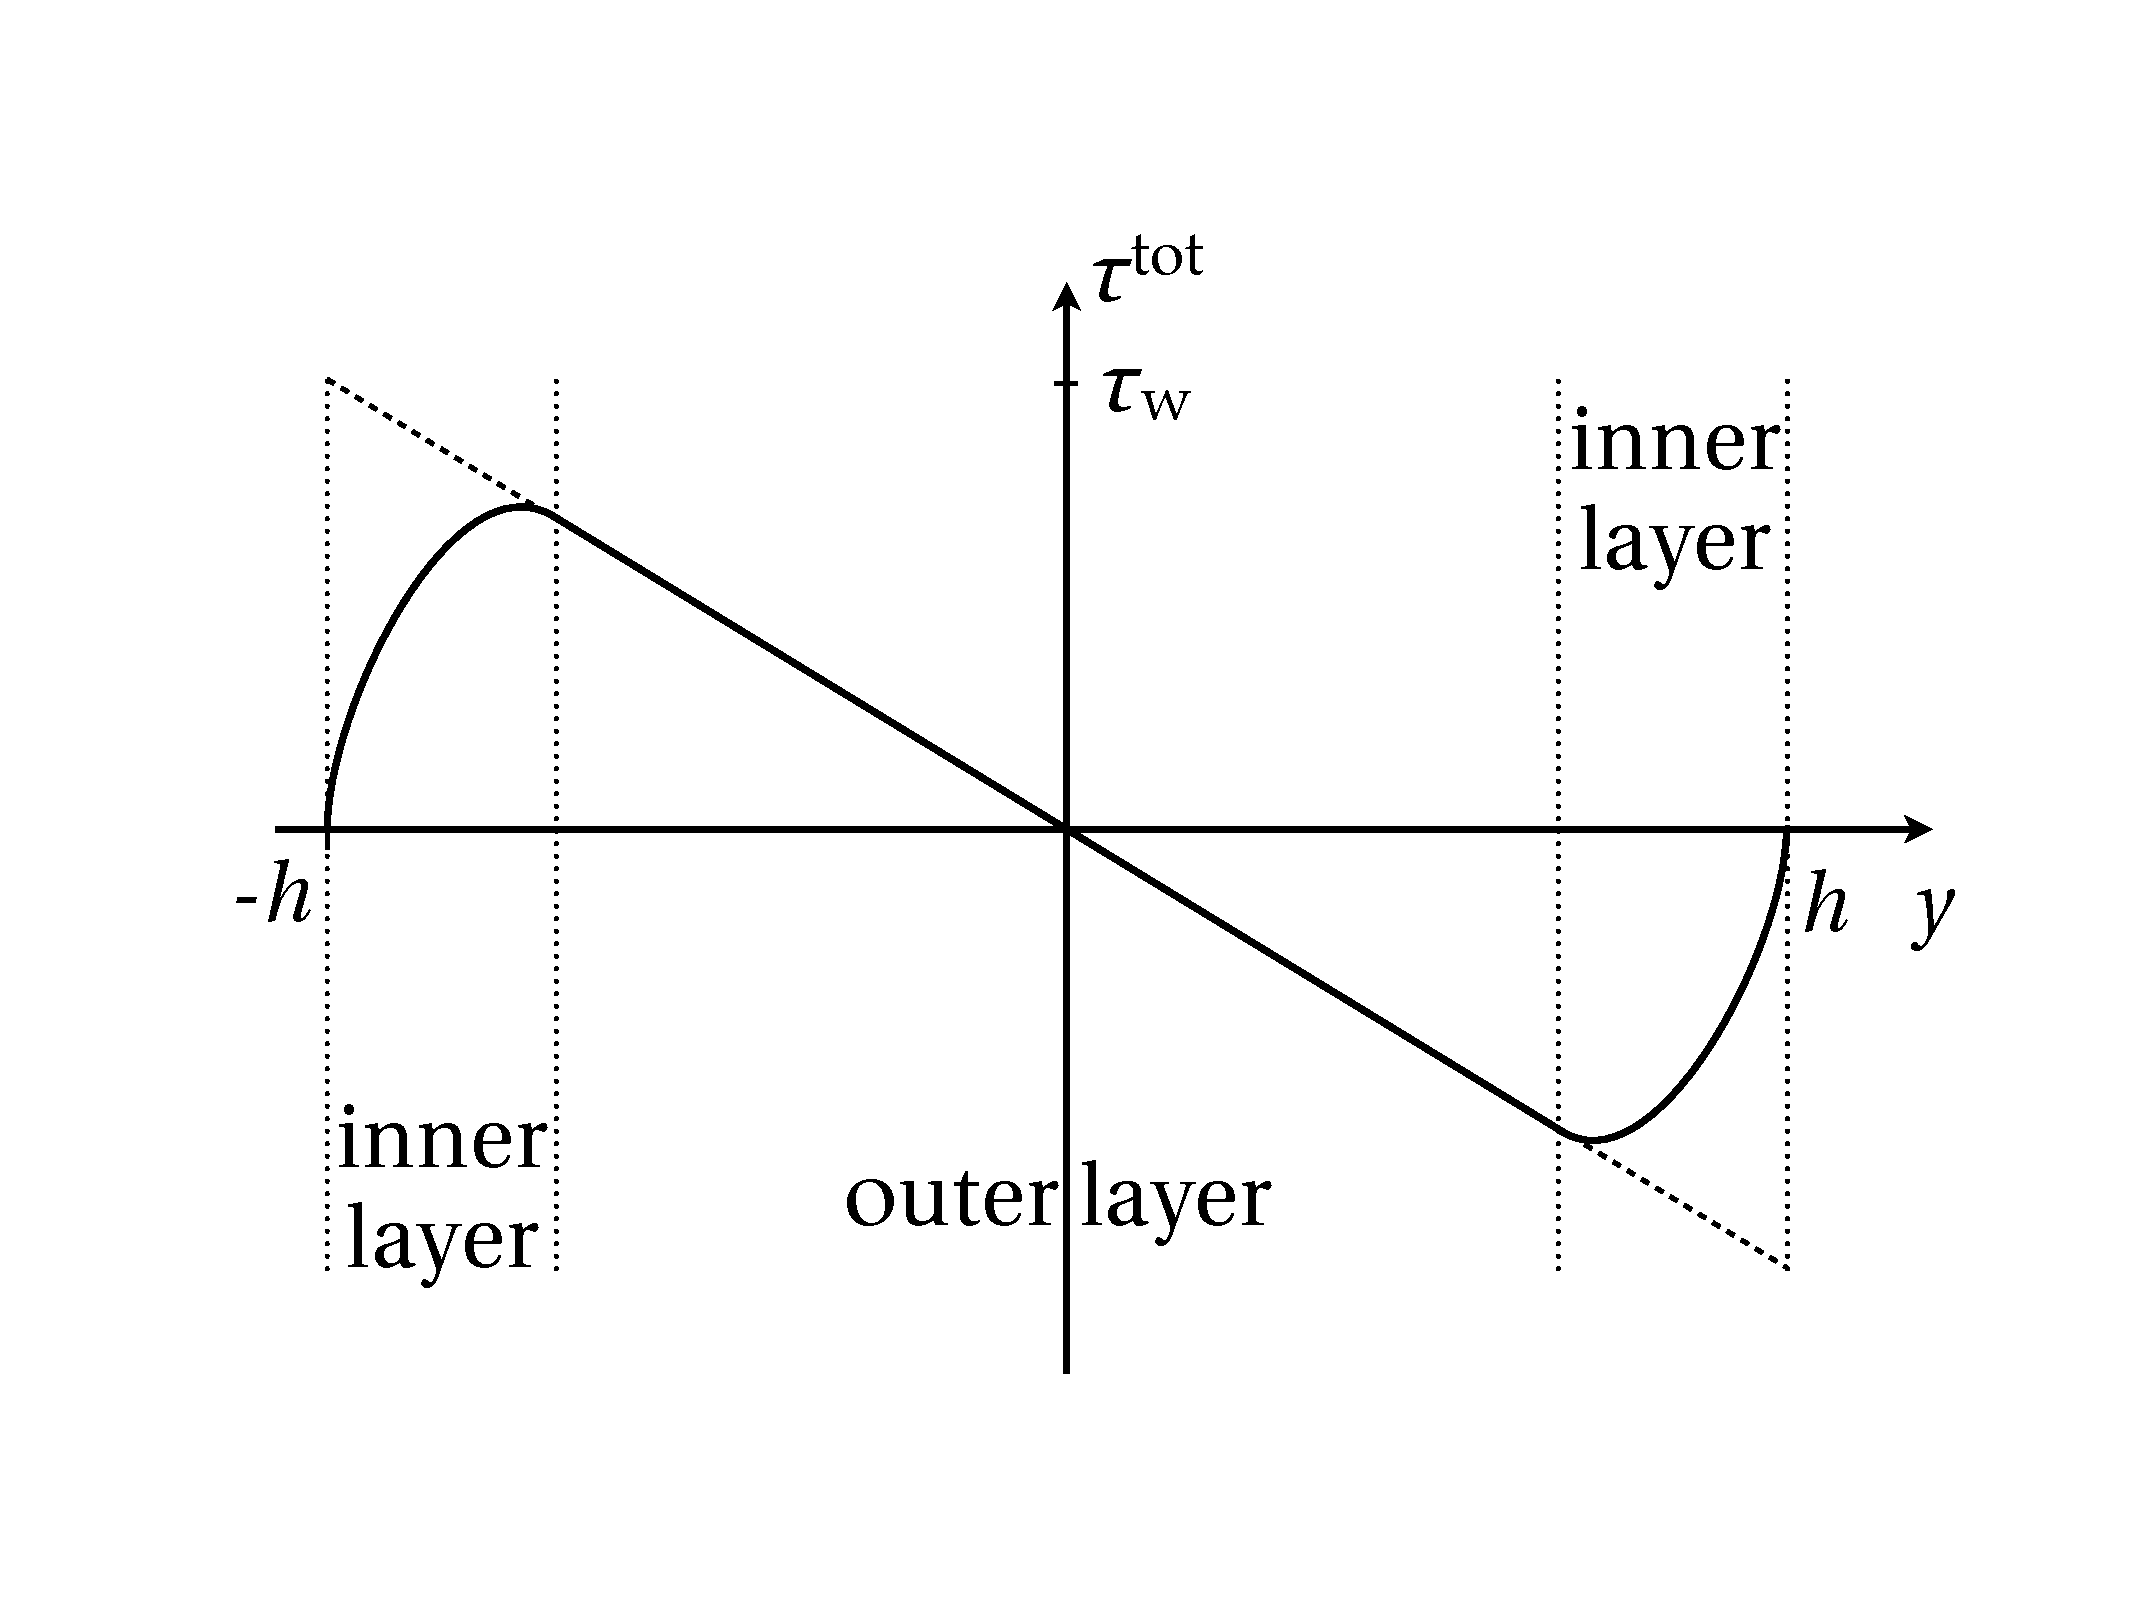
\includegraphics[scale=0.25]{ch4/6}
		\captionof{figure}{}
		\label{fig:4.6}
		\end{minipage}
		\begin{minipage}{0.49\textwidth}
		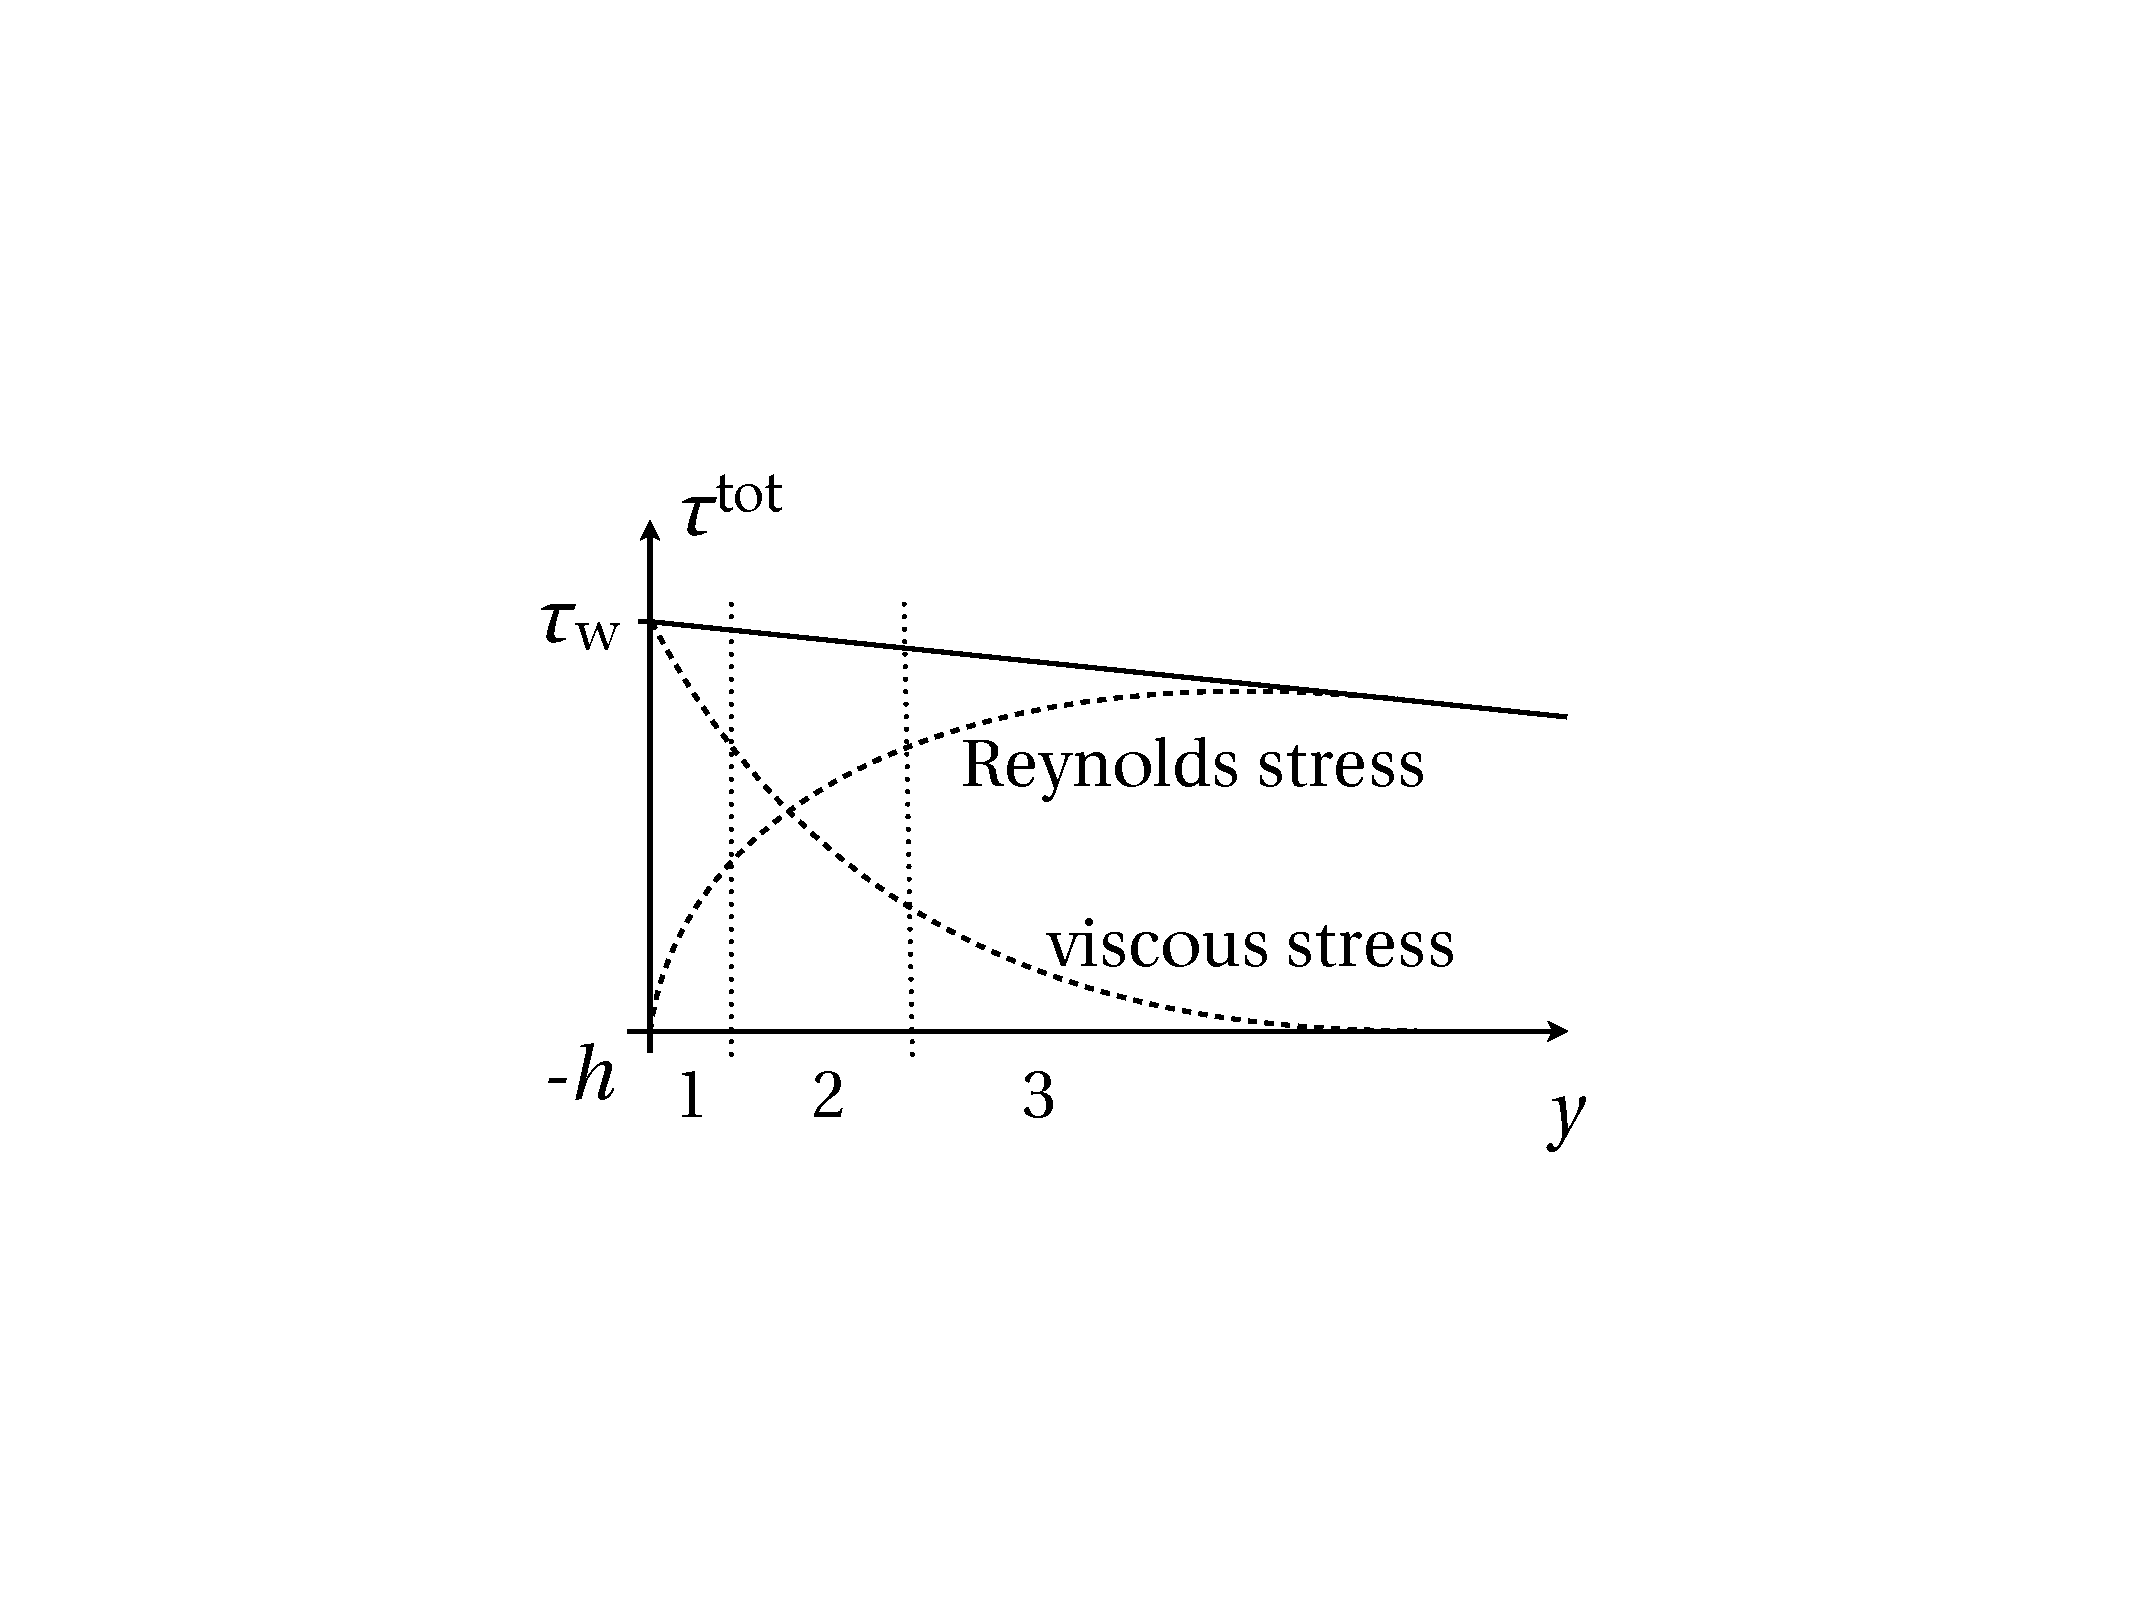
\includegraphics[scale=0.41]{ch4/7}
		\captionof{figure}{}
		\label{fig:4.7}
		\end{minipage}
		\end{center}
		
		The channel can be decomposed in several zones, namely the central zone where the total stress is nearly only the Reynold stress, there is hardly no conrtibution of the viscous stress. Then there is a region close to the wall where this last becomes dominant. The reason why the velocity profile is dependent of the Re number is that these two stresses doesn't vary in the same way with Re. \autoref{fig:4.6} represents the Re stress, the totally linear one beeing the total stress, so the viscous stress is null in the center whereas it increases near the wall (where Re stress decreases). We decompose the channel in an \textbf{outer zone }where $\tau _{21}^{tot} \approx \tau _{21} ^R = -\rho \langle u_1'u_2' \rangle$ and an \textbf{inner zone} where both stresses are significant. \autoref{fig:4.7} consists in a zoom on the left inner zone. \\
		
		We will now use dimensional analysis to find the velocity profile in the two regions. Let say that the average velocity at a point on the channel is a function of 
		\begin{equation}
			\langle u \rangle = f\left(y, \sqrt{\frac{\tau _{wall}}{\rho}} = u_{\tau}, \nu , u_c , h\right)
		\end{equation}
		Depending on the region, this function will change 
		\begin{equation}
			inner :  \langle u \rangle = f\left(y, \sqrt{\frac{\tau _{wall}}{\rho}} = u_{\tau}, \nu, \cancel{u_c}, \cancel{h}\right) \qquad outer : \langle u \rangle = f\left(y, \sqrt{\frac{\tau _{wall}}{\rho}} = u_{\tau}, \cancel{\nu}, u_c , h\right)
		\end{equation}
		where $u_\tau$ is the friction velocity. 

	\subsection{Inner zone (smooth wall)}
		If we look at our reduced function, this involves 4 quantities and 2 physical dimensions, leading to two dimensionless groups 
		\begin{equation}
			u^+ \equiv \frac{\langle u \rangle}{u_\tau} = f\left(Re = \frac{y u_\tau }{\nu}\equiv y^+\right)
		\end{equation}		 
		where $u^+$ and $y^+$ are the wall units, notation in litterature for these dimensionless groups. The inner zone can be decomposed into three sublayer as indicated on \autoref{fig:4.7} :\\
		\begin{itemize}
			\item[•] \textbf{the viscous sublayer (1) :} very close to the wall, where $\langle \tau _{21} ^V \rangle \gg \langle \tau _{21} ^R \rangle $
			\item[•] \textbf{the buffer layer (2) :} the transition layer where $\langle \tau _{21} ^V \rangle \approx \langle \tau _{21} ^R \rangle $ 
			\item[•] \textbf{the overlap layer (3) :} where $\langle \tau _{21} ^V \rangle \ll \langle \tau _{21} ^R \rangle $
		\end{itemize}
		
		\subsubsection{Viscous sublayer (1)}
			This layer is so small and close to the wall that 	
			\begin{equation}
			\begin{array}{cccc}
				&\tau _{21} ^{tot}(y)= \mu \frac{\D \langle u \rangle }{\D y} \approx \tau _{wall}  &\Leftrightarrow  &\frac{\mu}{\rho}\frac{\D \langle u \rangle }{\D y} = \frac{\tau _{wall}}{\rho} = u_\tau ^2\\
				\Leftrightarrow &\nu \langle u \rangle = u^2_{\tau} y &\Leftrightarrow  &\frac{\langle u \rangle }{u_\tau} = \frac{u_\tau y}{\nu}
			\end{array}
			\end{equation}
			This means that here we have the final result 
			\begin{equation}
				u^+ = y^+
			\end{equation}
			
		\subsubsection{Overlap layer (3)}
			There viscosity does not play a role. In other words, we expect that 
			\begin{equation}
				\frac{\D \langle u \rangle}{\D y} = f'\left(y, u_\tau , \cancel{\nu}\right) \qquad \Rightarrow \frac{y}{u_\tau}\frac{\D \langle u \rangle}{\D y} \approx cst = \frac{1}{\kappa}.
			\end{equation}
			So if we make appear the wall notations, we have
			\begin{equation}
				\frac{u_\tau^2}{\nu}\frac{\D u^+ }{\D y^+} = \frac{1}{\kappa}  \frac{u_\tau}{y} \qquad\Rightarrow \frac{\D  u^+}{\D y^+} = \frac{1}{\kappa}\frac{\nu}{yu_\tau} = \frac{1}{\kappa y^+} \qquad \Rightarrow u^+ = \frac{1}{\kappa}\ln y^+ + B.
				\label{eq:4.37}
			\end{equation}
						
		\begin{wrapfigure}[8]{l}{5cm}
		\vspace{-5mm}
		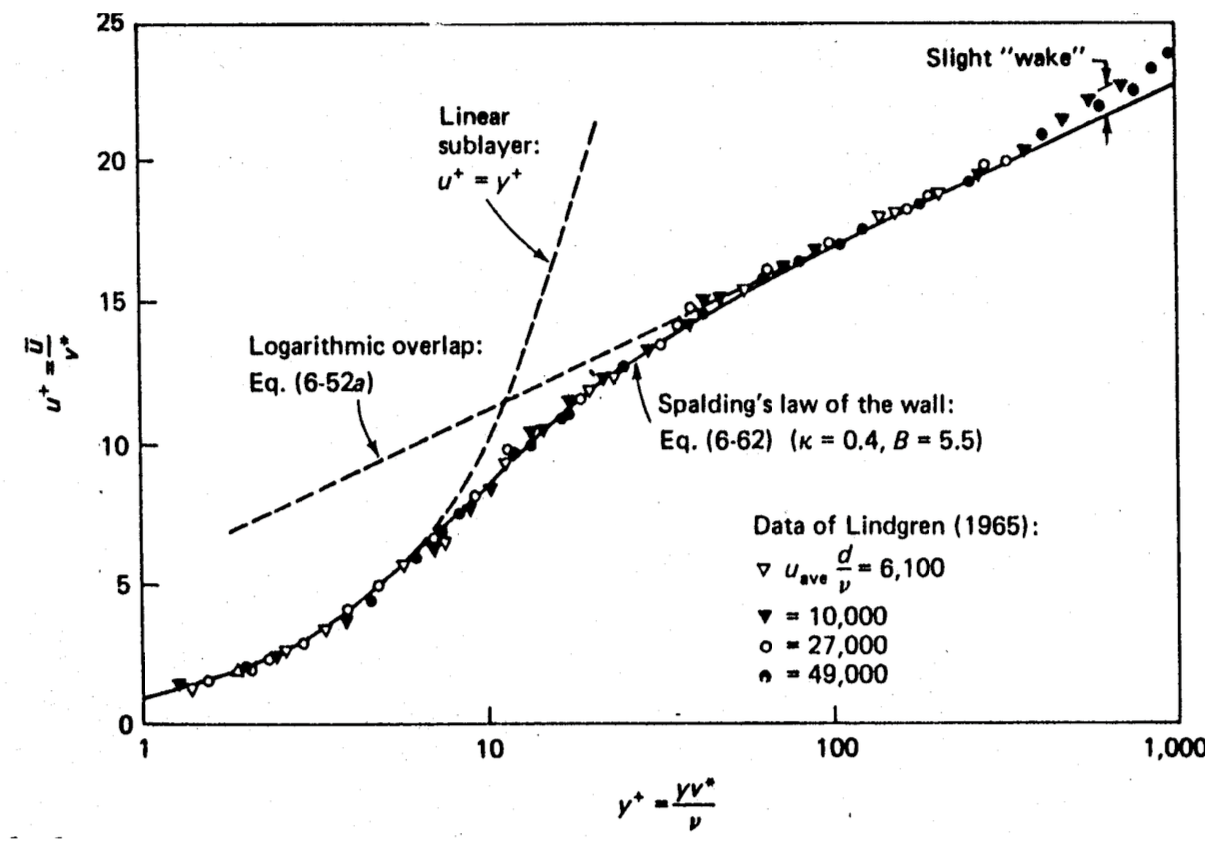
\includegraphics[scale=0.2]{ch4/8}
		\captionof{figure}{}
		\label{fig:4.8}
		\end{wrapfigure}
		This is theory, let's check what theory says about. When we look at the diagram, our theory matches roughly with the linear (in $\log$) for $50\leq y^+ \leq 500$. For the viscous sublayer represented by the exponential, the curves matches till $y^+ \approx 5$ wall units. That's very small (1/10 - 1/100 of the overloop). There is a smooth transition between the two curves. 
		
	\	\\ \subsubsection{Buffer layer (2)}
			The idea is to rewrite the expression of the two zones but with $y^+ = f(u^+)$ 
			\begin{equation}
			\begin{aligned}
				&viscous \ layer : y^+ = u^+\\
				&overloop \ layer : y^+ =  \exp (\kappa(u^+ - B))= \exp (\kappa u^+)\exp (-\kappa B)
			\end{aligned}
			\end{equation}
			We can have a good transition between the two by 
			\begin{equation}
				y^+ = u^+ + \exp (-\kappa B)\left[ \exp(\kappa u^+) - \underbrace{\left( 1 + \kappa u^+ +  \frac{(\kappa u^+)^2}{2}  +  \frac{(\kappa u^+)^3}{6}\right)}_{taylor \ serie \ expansion \ of\ \exp(\kappa u^+)}\right]
			\end{equation}
			Indeed when $\kappa u^+$ is small, the second part will be negligible regarding $u^+$ and for high, we found the overlap layer. To have the smooth transition, only two terms are enough but taking more leads to a best fitting with the practice. 
			
	
	\subsection{Inner zone (rough wall)}
		The wall are never exactly smooth in rality. We already discussed that to have exact similarity between the model and the prototype we must have the same relative rougness ($\lambda /L$). Let's see the effect on velocity profile. In practice it is impossible to do an exhaustive study because of the number of parameters. There is also various forms of roughness: \\
		
		\begin{itemize}
			\item[•] \textbf{uniform sand roughness:} when you blew sand particles on a paper for example 
			\item[•] \textbf{non uniform sand roughness:} when particles have different scale and form
			\item[•] \textbf{periodic roughness:} this can be obtained for example if we put wires or square ribs at regular interval. \\
		\end{itemize}
		
		We will consider the first one. In the overlap layer, we expect that \eqref{eq:4.37} remains correct but B will be function of $k^+$ which is $k$, the hight of the grains, in wall units (divided by the inner zone length scale)
		\begin{equation}
			u^+ = \frac{1}{\kappa}\ln y^+ + B_1(k^+) \qquad with \qquad k^+ =k \frac{u_\tau}{\nu}
		\end{equation}
		We expect that roughness will slow down the fluid meaning that $B_1(k^+) < B$. We can rewrite our equation as 
		\begin{equation}
			u^+ = \frac{1}{\kappa}\ln y^+ + B - \Delta u^+ (k^+) \qquad where \qquad \Delta u^+ (k^+) = B - B_1(k^+)
		\end{equation}
		where $\Delta u^+$ is the velocity deficit, expected to be $>0$.\\
		
		\begin{wrapfigure}[8]{l}{6.5cm}
		\vspace{-5mm}
		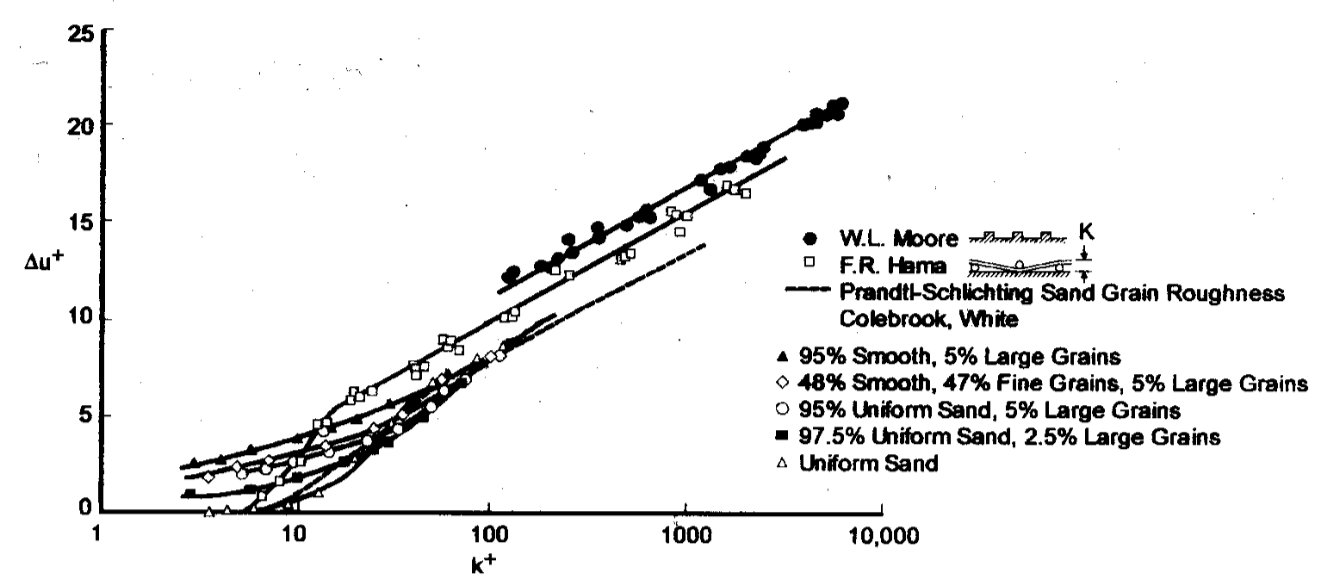
\includegraphics[scale=0.27]{ch4/9}
		\captionof{figure}{}
		\label{fig:4.9}
		\end{wrapfigure} 
		In experiments we see indeed that $\Delta u^+$ is a function of $k^+$ and depends on the type of roughness. In which we concerns, we have to look to the triangles. The first observation is that $\Delta u^+ = 0$ for $k^+ \leq 5$, so if the roughness is such that the hight doesn't exceed 5 in wall units, the fluid behaves exactly as the wall was smooth : \textbf{hydraulically smooth regime}. Let's remind that 5 is the upper limit of the viscous sublayer. The conclusion is that, as long as the grains remains barried within the viscous sublayer, roughness does not influence the average velocity profile. For non uniform roughness, there are bigger grains that goes throw this limit. 
		The second observation is that for higher $k^+$ ($\geq 80$) on the logarithmic axis $\Delta u^+$ respect a line of constant slope 
		\begin{equation}
			\Delta u^+ =  \frac{1}{\kappa} \ln k^+ + B_3 \qquad k^+ \geq 80 
		\end{equation}
		This means that the velocity profile in this zone is 
		\begin{equation}
			u^+   = \frac{1}{\kappa} \ln y^+ + B - \left(  \frac{1}{\kappa} \ln k^+ + B_3 \right) 
 		= \frac{1}{\kappa} \ln \frac{y^+}{k^+} + B - B_3  = \frac{1}{\kappa} \ln \frac{y}{k} + B - B_3 
		\end{equation}
		We see that the appropriate length scale changes from $\nu / u_\tau$ to beeing $k$ itself and this is called the \textbf{fully rough regime} where we can make another manipulation for $u^+$ 
		\begin{equation}
		\begin{array}{c}
			u^+ = \frac{1}{\kappa}\ln y^+ + B - \Delta u^+ (k^+)  = \frac{1}{\kappa}\ln \frac{y^+}{k^+} + \underbrace{B + \frac{1}{\kappa} \ln k^+ - \Delta u^+ (k^+)}_{B_2(k^+)} \\
			where \\\\
			k^+ \leq 5 \quad B_2(k^+) \approx B+\frac{1}{\kappa}\ln k^+ \qquad k \geq 80 \quad B_2(k^+) \approx B-B_3
		\end{array}
		\end{equation}
		
		\begin{wrapfigure}[10]{l}{5.8cm}
		\vspace{-2mm}
		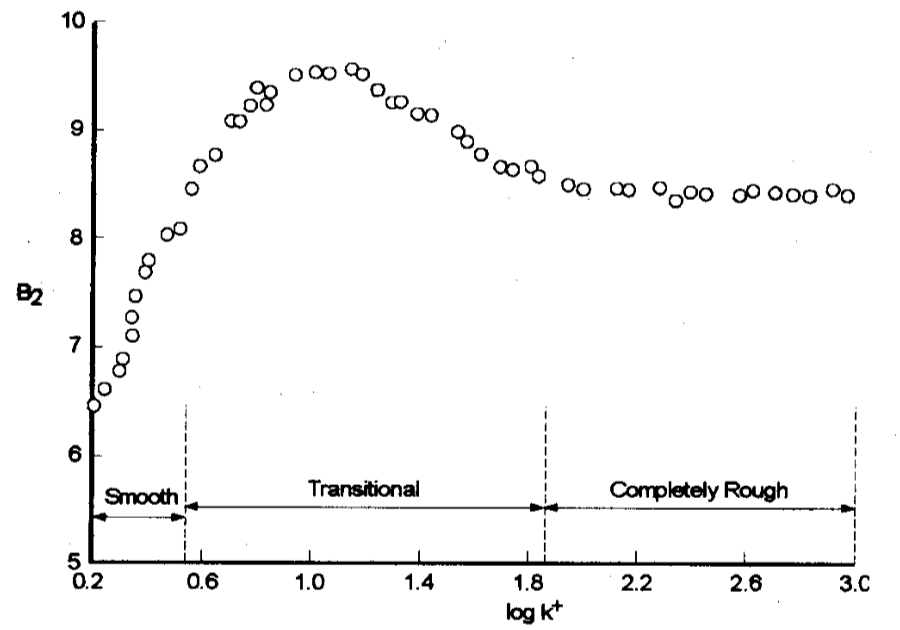
\includegraphics[scale=0.35]{ch4/10}
		\captionof{figure}{}
		\end{wrapfigure} 
		This is shown on this diagram where we have a linear curve for $k\leq 5$ giving $B = 5.5$ (y axis) and then the constant area ($k\leq 80$). Notice that we have an overshoot in the transitional zone between the two, this is important to see. Let's see what happens in the irregular roughness case. If we come back to \autoref{fig:4.9}, we can see that in the fully rough regime, the irregular curve corresopnds to a simple shift of the regular one. In order to approach this second case, let's compute $B_3$ for uniform sand roughness by extrapolating $B - B_2 = 5.5 - 8.5 = -3$. The equivalent sand roughness will be defined in such a way that we have the same $\Delta u^+$ in the fully rough regime where $B_S$ is the universal value of -3 
		\begin{equation}
			\Delta u^+ = \frac{1}{\kappa} \ln k^+ + B_3 = \frac{1}{\kappa} \ln k_S^+ + B_{3S} \qquad \Leftrightarrow \frac{1}{\kappa} \ln \frac{k_S^+}{k^+} = \frac{1}{\kappa} \ln \frac{k_S}{k} = B_3-B_{3S}.
		\end{equation}
		
	
	\subsection{Outer zone}
		Let's remind that we assumed 
		\begin{equation}
			\langle u \rangle = f(y,u_\tau , u_c , h) \qquad \mbox{or for a boundary layer: } u_c \mbox{ outer flow velocity and } h\rightarrow \delta 
			\label{eq:4.46}
		\end{equation}

		\begin{wrapfigure}[10]{r}{4cm}
		\vspace{-5mm}
		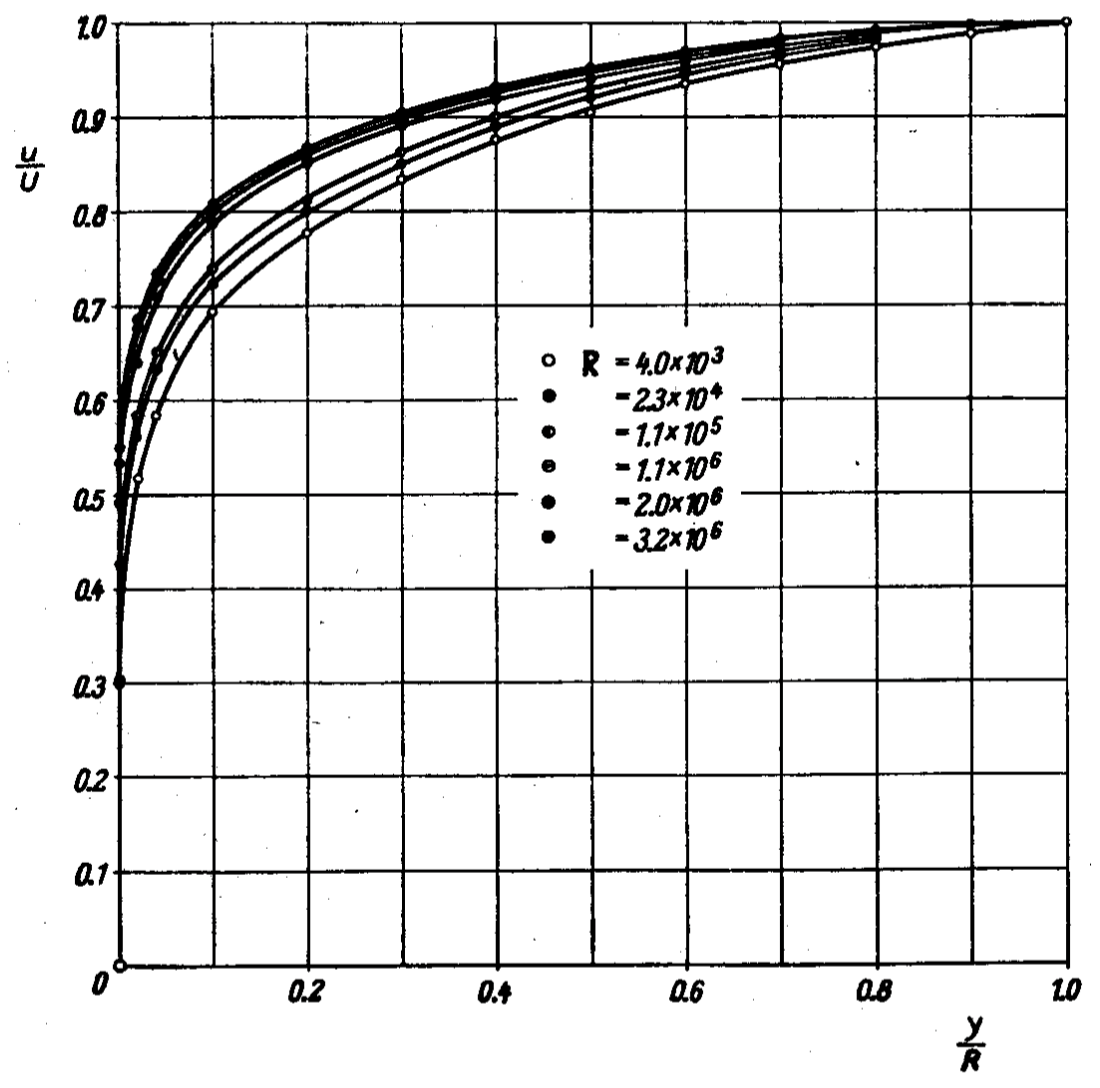
\includegraphics[scale=0.20]{ch4/11}
		\captionof{figure}{}
		\end{wrapfigure} 
		To determine what this function should be, let's go to the velocity profile in the pipe where we started from to be guided from the curves. These are more or less flat depending on the Reynolds number whith $u/u_c \rightarrow 1$ ($u_c$ velocity at the center of the pipe). Let's imagine that we plot now $1-\frac{\langle u \rangle}{u_c} = \Delta u /u_c$ in function of $y/R$, 1 will become 0 and  $0 \rightarrow 1$, the graph will be reversed (\autoref{fig:4.12} left). The curves seems to be similar, so maybe I take the velocity deficit of the half hight $\Delta u(0.5)/u_c$ which depends on Reynolds number and plot that for $\frac{u_c - \langle u \rangle}{u_c}\frac{u_c}{\Delta u}$ (\autoref{fig:4.12} center). When this = 1, $y/r = 0.5$ and we see that it fall on the same curve as \autoref{fig:4.12} left but we get a single curve. This means that 
		\begin{equation}
			\frac{u - \langle u \rangle}{\Delta u} = f\left(\frac{y}{R}\right)
		\end{equation}
		where the only scale that doesn't appear based on \eqref{eq:4.46} is $u_\tau$. So if we plot $\frac{u_e  - \langle u \rangle}{u_\tau} = f\left(\frac{y}{R}\right)$ ($u_e$ max velocity at the center) we will obtain a single curve shown on \autoref{fig:4.12} right. 
\begin{figure}[h]
\begin{center}
      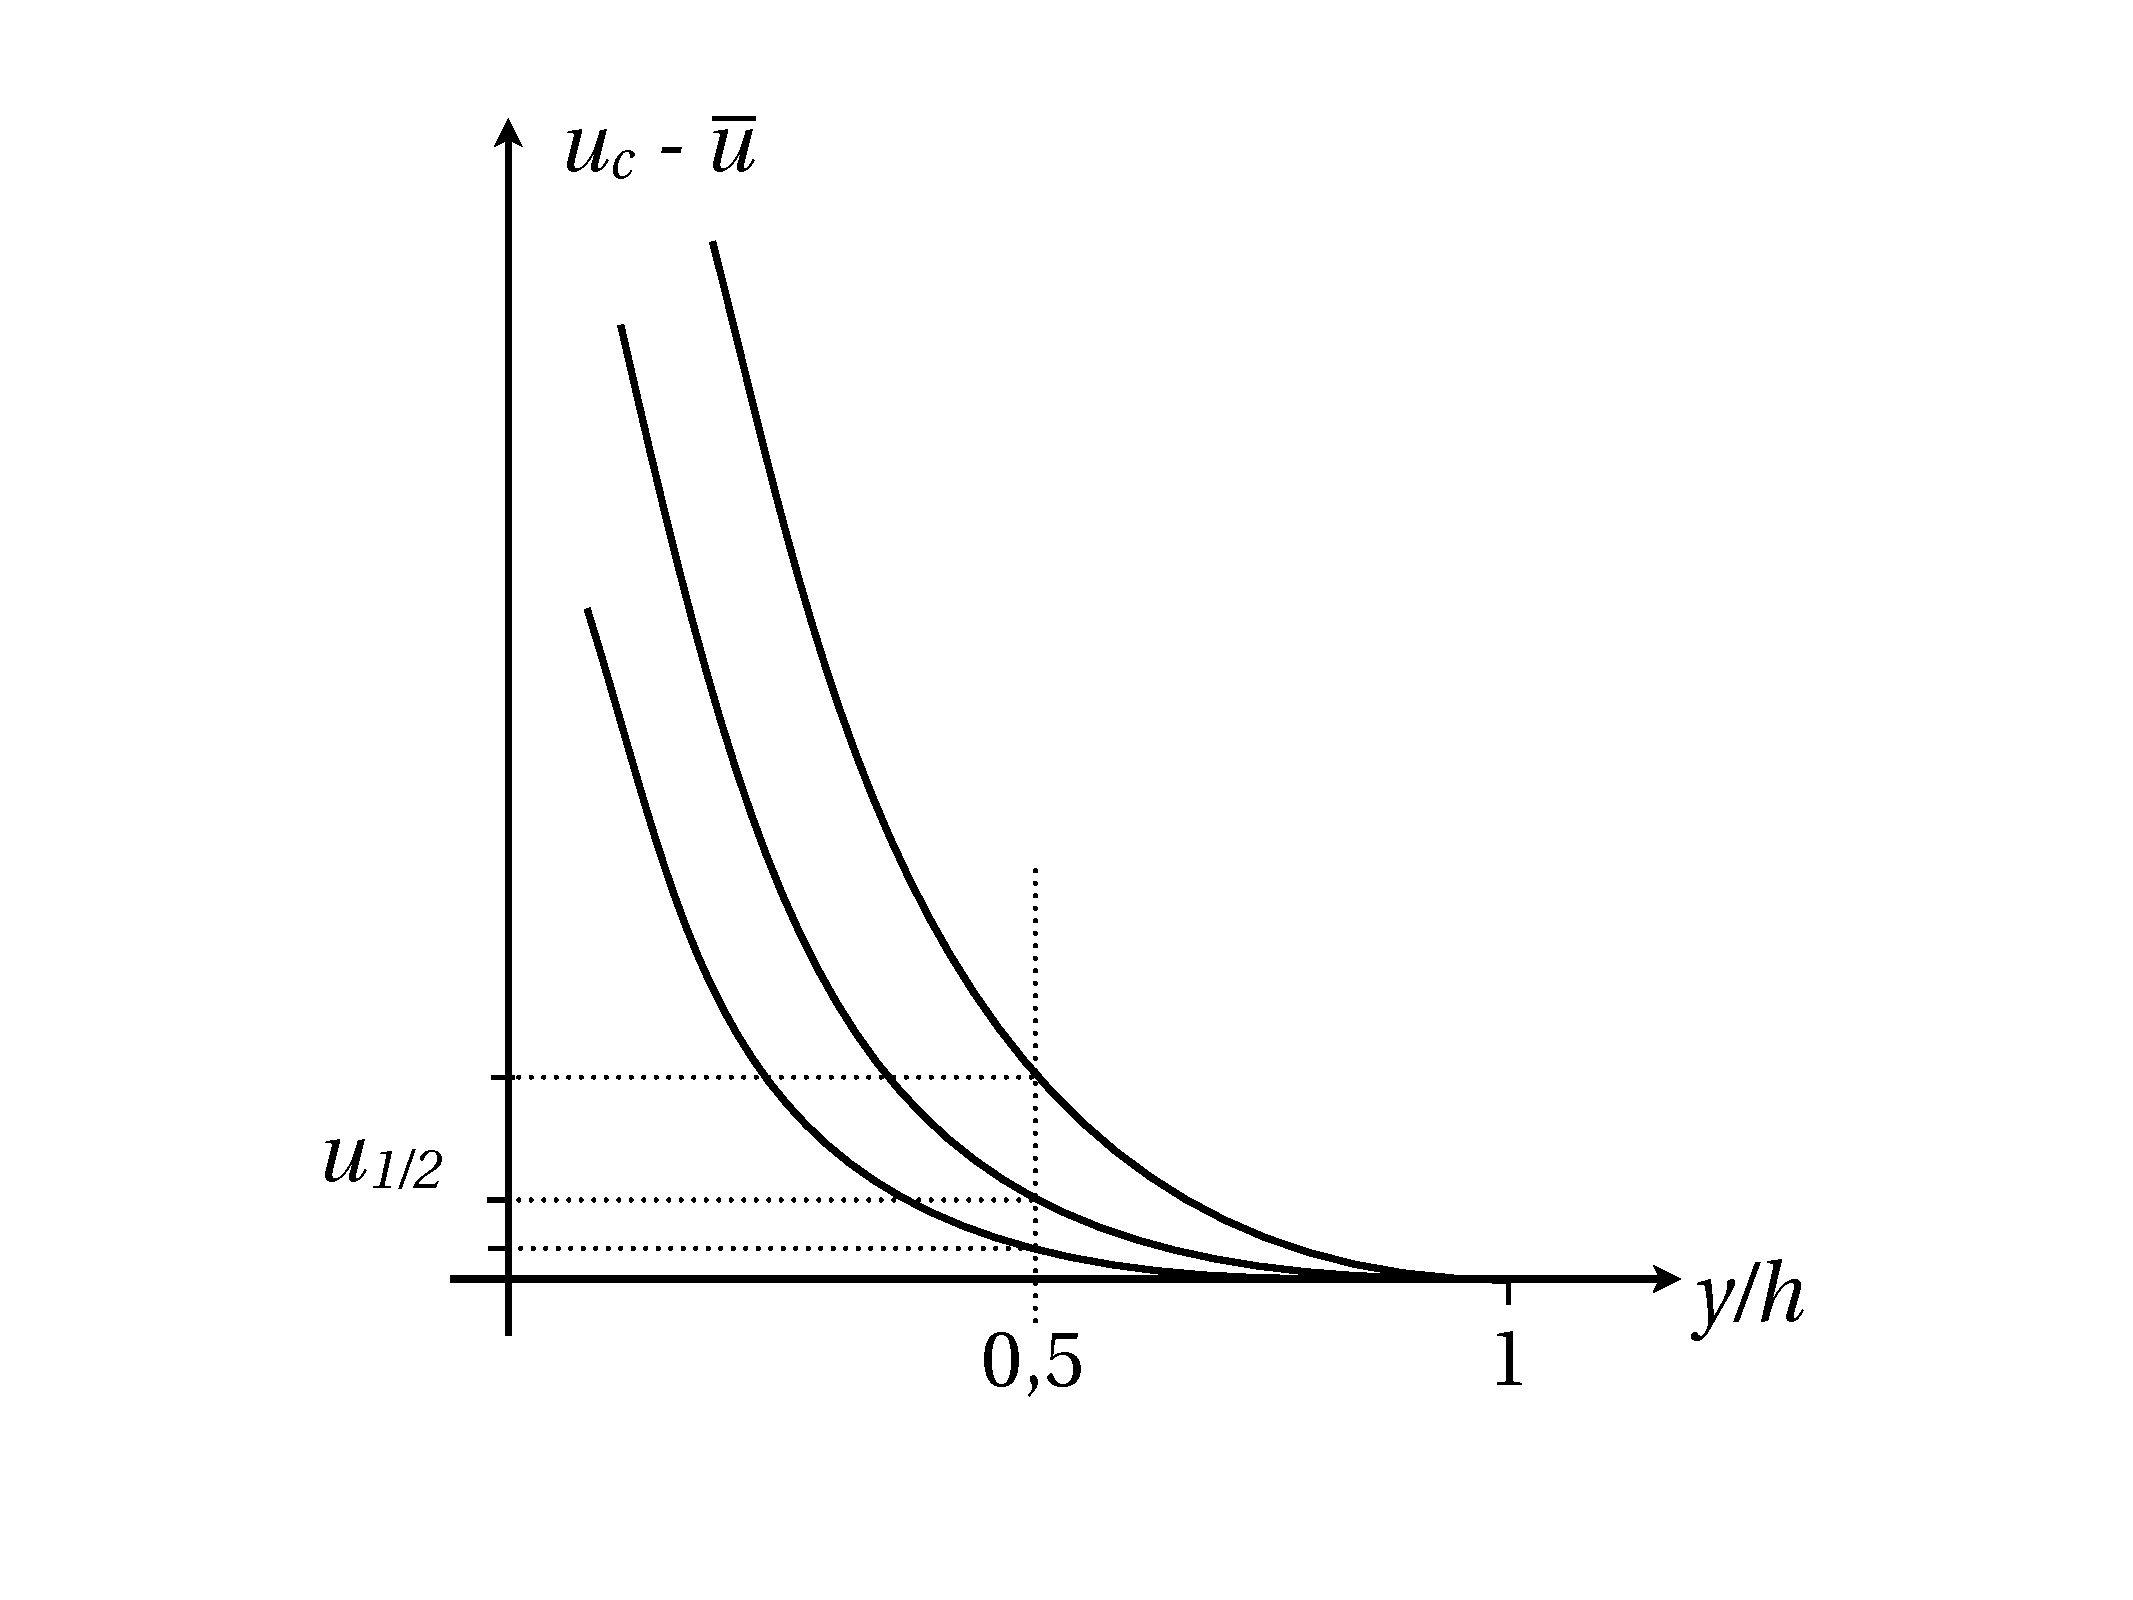
\includegraphics[scale=0.19]{ch4/12} \quad  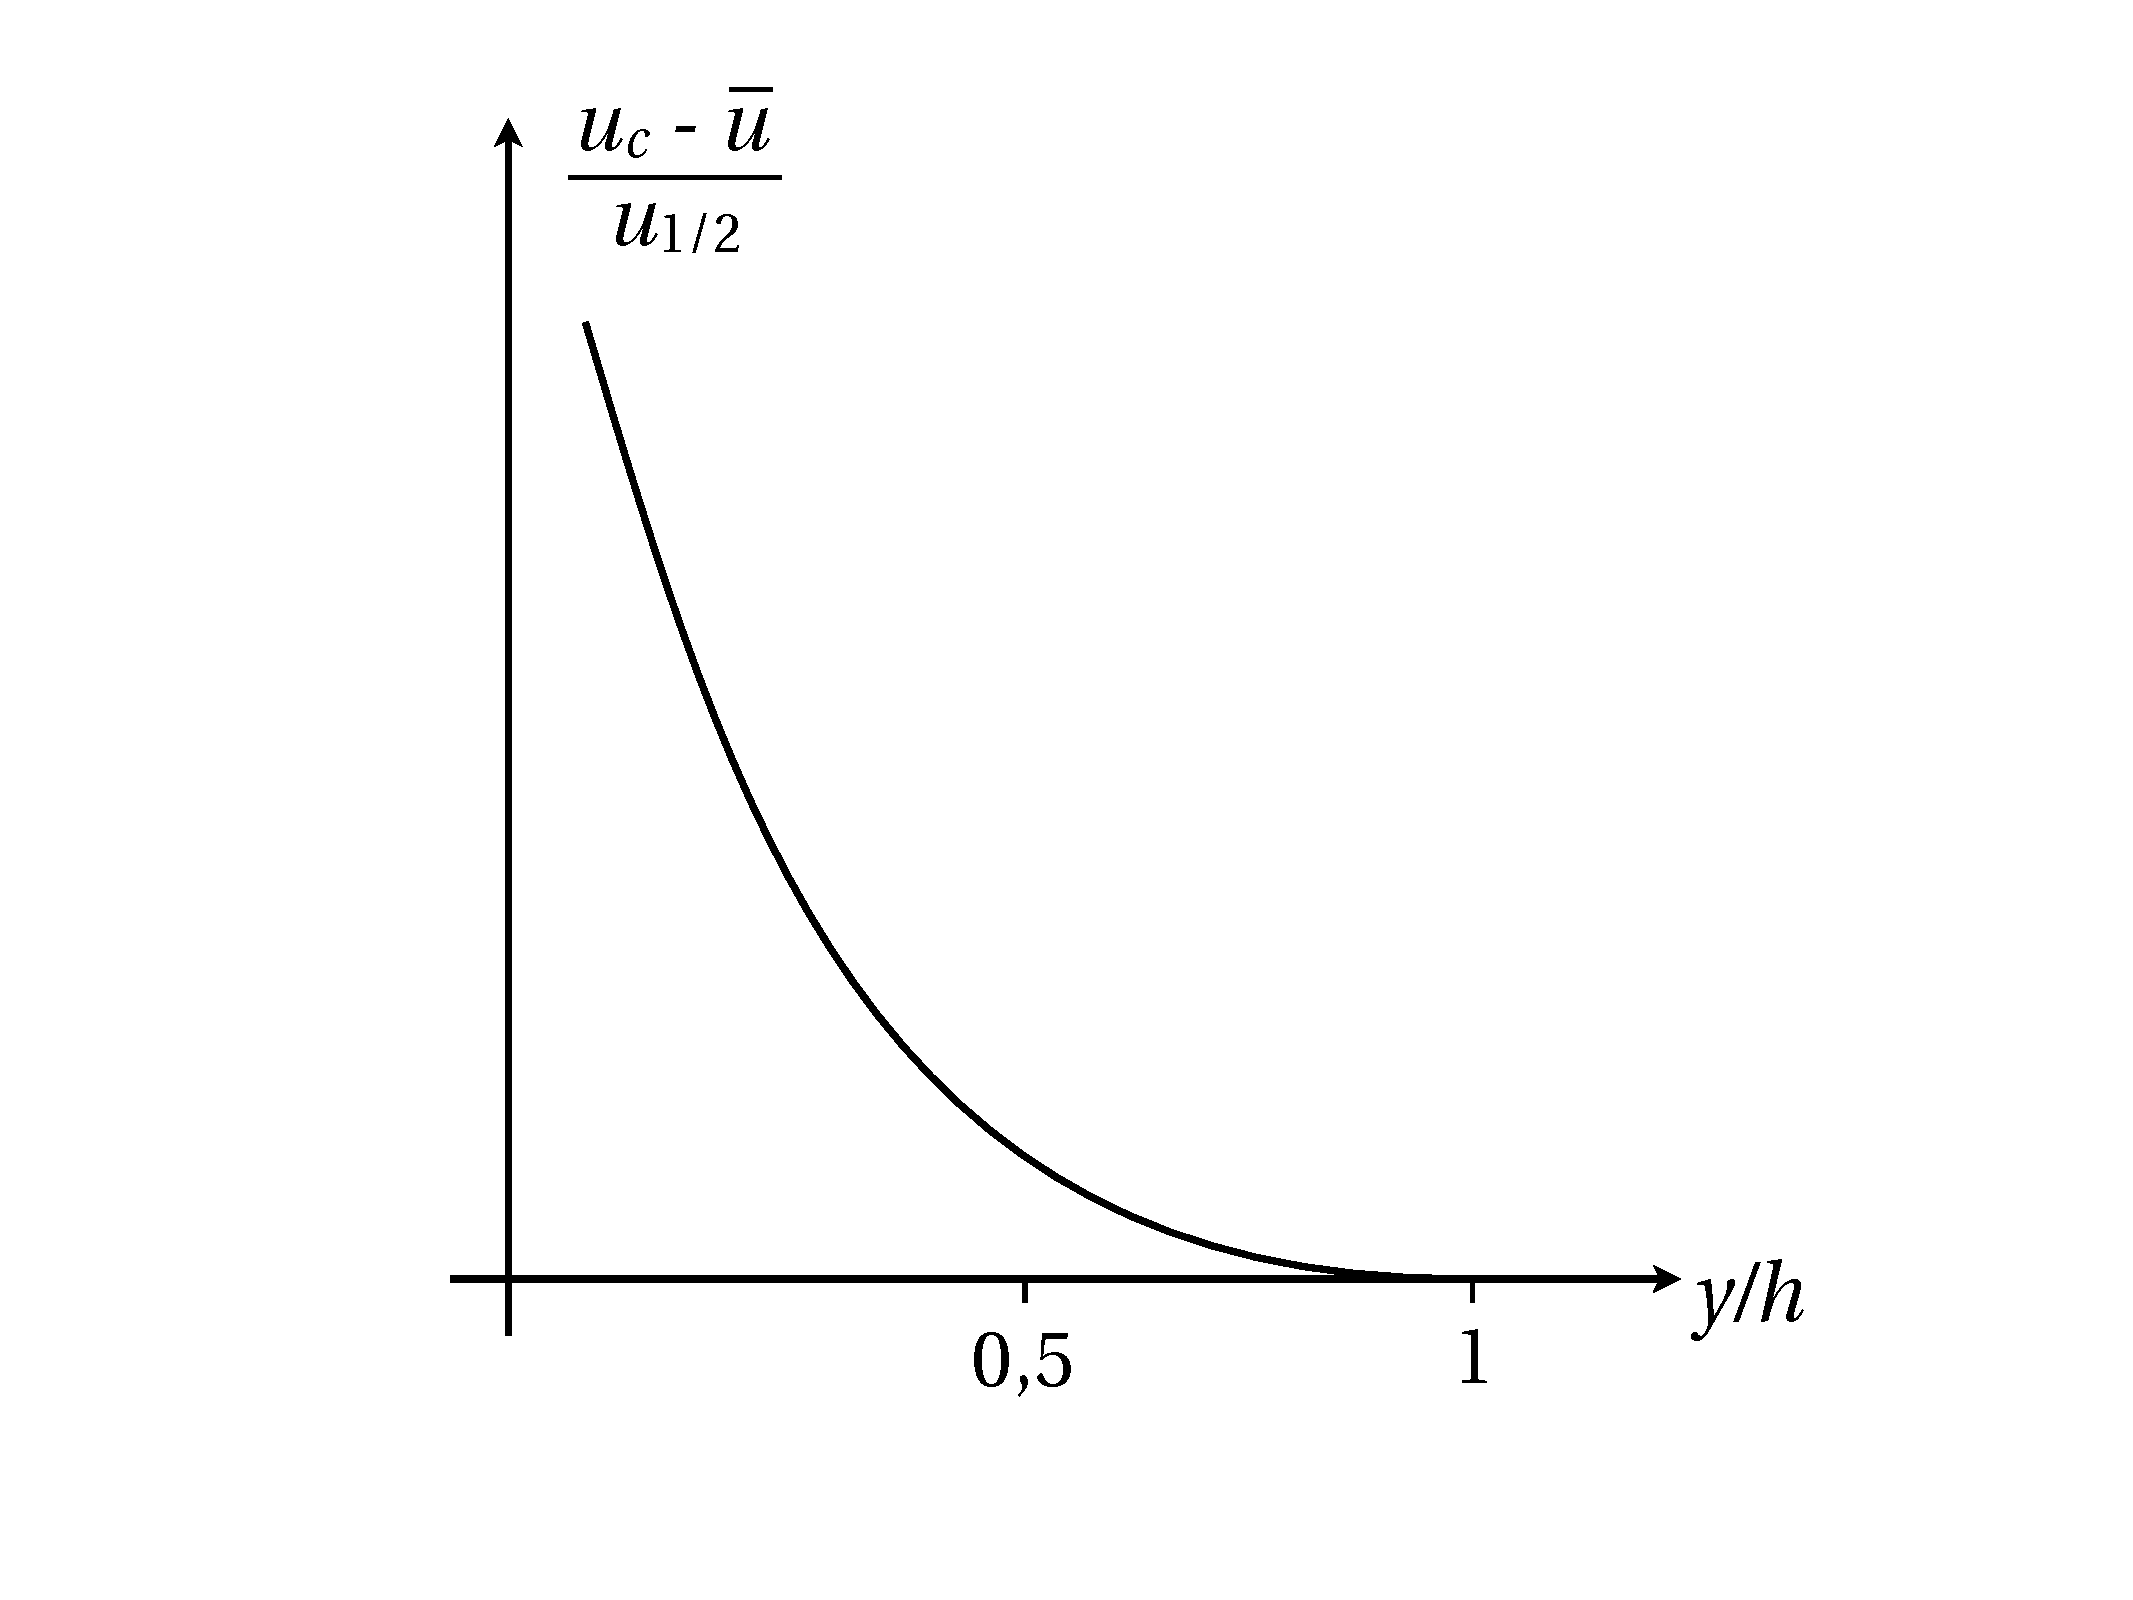
\includegraphics[scale=0.185]{ch4/13} \quad 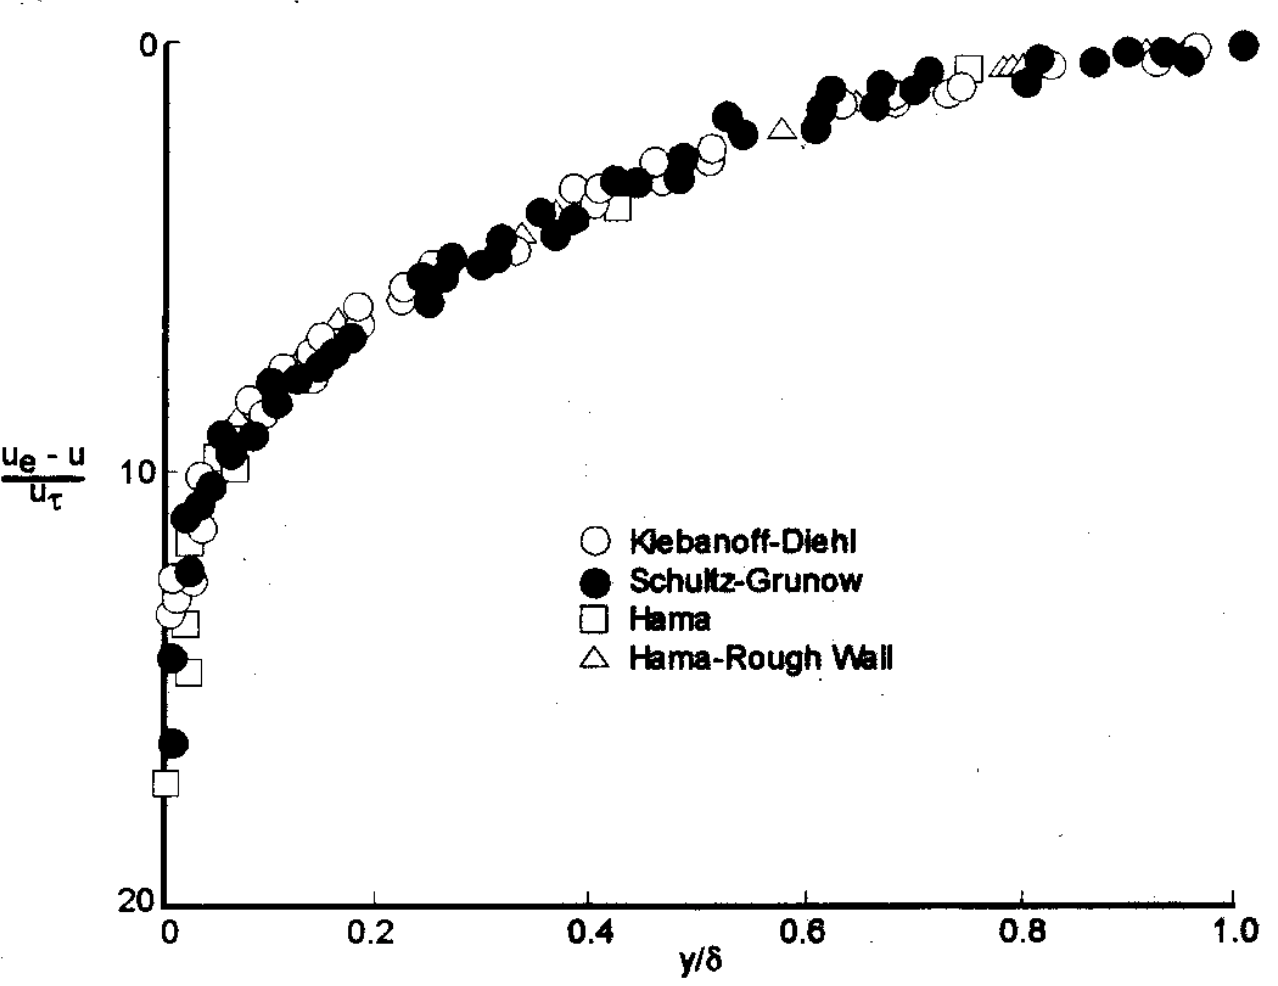
\includegraphics[scale=0.24]{ch4/14}
\captionof{figure}{}
\label{fig:4.12}
\end{center}
\end{figure}

		Interestingly enough, the logarithmic low is compatible with the outer scaling 
		\begin{equation}
			\frac{\langle u \rangle }{u_\tau} = u^+ = \frac{1}{k}\ln y^+ + B
		\end{equation}
		But what's $u_e /u_\tau$? We know that 
		\begin{equation}
			u_\tau = \sqrt{\frac{\tau _{wall}}{\rho}} \qquad \Rightarrow \frac{u_\tau}{u_e} = \sqrt{\frac{\tau _{wall}}{\rho u_e^2}} = \sqrt{\frac{C_f}{2}} \qquad \Rightarrow \frac{u_e}{u_\tau} = \sqrt{\frac{2}{C_f}} 
		\end{equation}
		where we define the \textbf{friction coefficient} $C_f = \frac{\tau _{wall}}{\rho u_e^2 /2}$ as we defined the pressure coefficient $\frac{p-p_\infty}{\rho \uinf ^2 /2}$. By combining the two last equation, we have
		\begin{equation}
		\begin{aligned}
			\frac{u_e - \langle u \rangle}{u_\tau} &= \sqrt{\frac{2}{C_f}} - \frac{1}{\kappa} \ln \left(\frac{yu_\tau}{\nu}\frac{\delta}{\delta}\right) - B = \sqrt{\frac{2}{C_f}} - \frac{1}{\kappa} \ln \frac{\delta u_\tau}{\nu} - B -\frac{1}{\kappa} \ln \frac{y}{\delta}\\
			&= cst -\frac{1}{\kappa} \ln \frac{y}{\delta}
		\end{aligned}		
		\end{equation}

		\begin{wrapfigure}[10]{l}{5.5cm}
		\vspace{-5mm}
		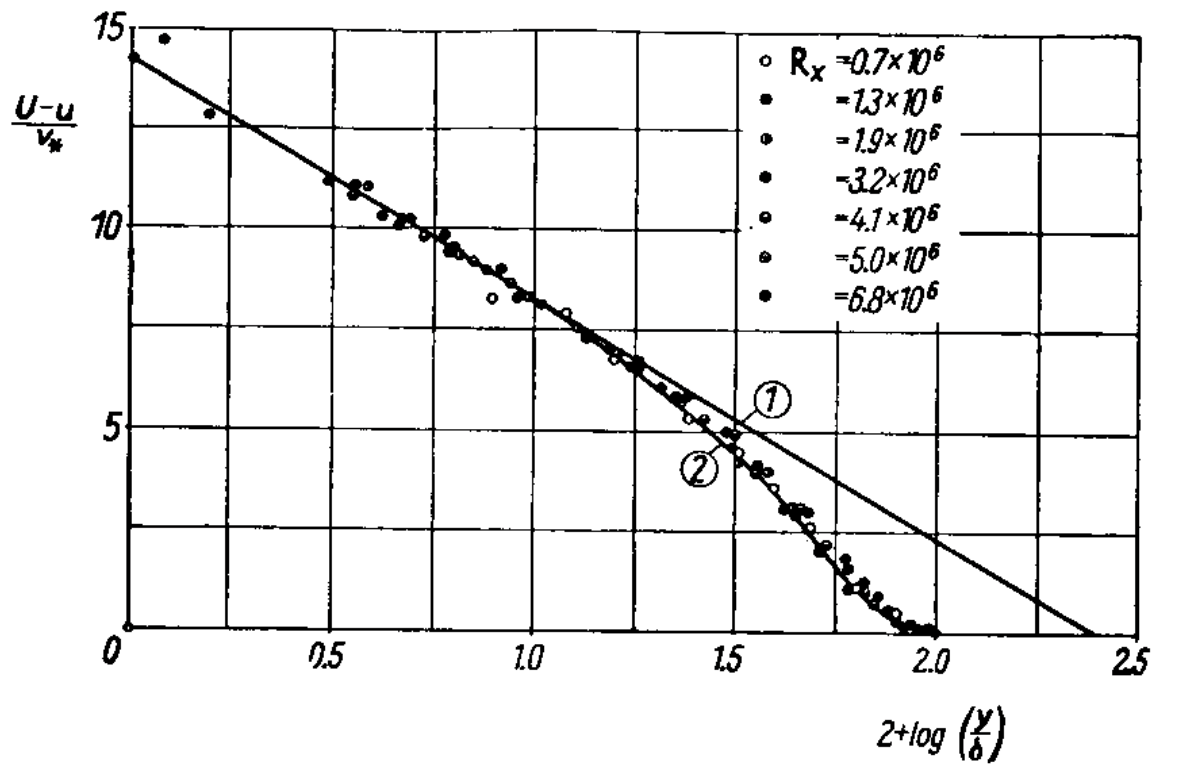
\includegraphics[scale=0.25]{ch4/15}
		\captionof{figure}{}
		\label{fig:4.13}
		\end{wrapfigure} 
		that confirms the previously founded relation. Wa can plot this in logarithmic scale that gives \autoref{fig:4.13}. We see that it obbeys the logarithmic law as in the overlap layer which is compatible with the inner and outer zone scaling. In fact we can rewrite our last equation as 
		\begin{equation}
			 \frac{u_e - \langle u \rangle}{u_\tau} = f\left( \frac{y}{\delta}\right) = cst -\frac{1}{\kappa} - g\left(\frac{y}{\delta} \right)
		\end{equation}
		where $g\left(\frac{y}{\delta} \right)$ is the deviation compared to the logarithmic law. Because of velocity deficit = 0 when $y/\delta =1$, it turns out that the cst = g(1). As conclusion, we found that the velocity profile is given by 
		\begin{equation}
			u^+ = \frac{1}{\kappa} \ln y^+ + B + g\left(\frac{y}{\delta} \right)
		\end{equation}
 		and this is observed on \autoref{fog:4.8} where we observe the deviation at the very right side of the figure. 
 		
 		\begin{wrapfigure}[9]{r}{5.4cm}
		\vspace{-5mm}
		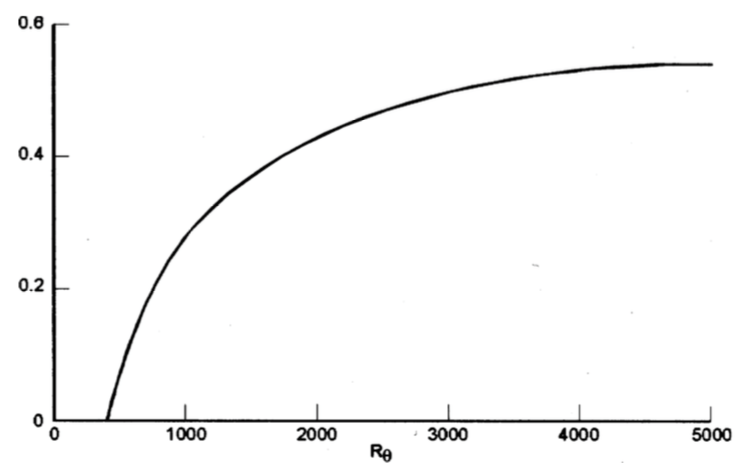
\includegraphics[scale=0.4]{ch4/16}
		\captionof{figure}{}
		\label{fig:4.16}
		\end{wrapfigure} 
		For the case of zero pressure gradient, Coles observed that the deviation from the logarithmic velocity profile $g\left(\frac{y}{\delta} \right)$ is similar to the velocity profile in a half-jet
or wake
\begin{equation}
	g\left(\frac{y}{\delta} \right) = \Pi(x)w \left(\frac{y}{\delta} \right) \approx \Pi(x)2\sin ^2 \left(\frac{\pi}{2}\frac{y}{\delta} \right) 
\end{equation}
      which was subsequently called the \textbf{law of the wake}. The coefficient $\Pi (x)$ is the amplitude of the wake, which varies slightly with Reynolds number as shown on Fig. 29, ultimately reaching a constant value equal to about 0.55 for $Re\theta > 5000.$
      
     \newpage
\section{Introduction to turbulent modelling}
	Let's remind the average Navier-Stokes equation 
	\begin{equation}
		\rho \left[ \frac{\partial \bar{u}_i}{\partial t} + \frac{\partial \overline{u_i u_j}}{\partial x_j} \right] = - \frac{\partial \bar{p}}{\partial x_i} + \frac{\partial }{\partial x_j} \Big[ \underbrace{\mu \ \left( \frac{\partial \bar{u}_i}{\partial x_j} + \frac{\partial \bar{u}_j}{\partial x_i} \right)}_{\tau^v_{ij}} - \underbrace{\rho \bar{u_i}' \bar{u_j}'}_{\tau_{ij}^t} \Big]
	\end{equation}
	There is still some unknowns, we will try to find equations describing these unknowns. It is possible, but the problem is that we introduce more unknowns than we had before, it doesn't solve the problem. This means that to close the system of equation, one of them has to stop at one stage and model the unkonown terms. One approach is to model directly the Reynold stresses as a function of the average flow quantities, this is called \textbf{first order closure approach}.  The other strategy is to retain the transport equations  for Reynolds stresses and to model the unknows in these equations, \textbf{second order closure model}. We will make an introduction with the first approach. The most corresponding method to this is Bousinesq approach or Eddy viscosity approach. The idea is to use a model analogous to viscous stresses. For these we have the \textbf{Newton's model} that says 
	\begin{equation}
		\tau _{ji} = \mu\big( \frac{\D u_i}{\D x_j} + \frac{\D u_j}{\D x_i}  \underbrace{- \frac{2}{3}\delta _{ij}\frac{\D u_k}{\D x_k}}_{=0 \mbox{ constant density}} \big) 
		\Rightarrow  - \rho \bar{u}_i' \bar{u}_j' = \mu_t \left( \frac{\partial \bar{u}_i}{\partial x_j} + \frac{\partial \bar{u}_j}{\partial x_i} \right) - \rho \underbrace{\overline{u'_k u'_k}}_{2k} \frac{\delta _{ij}}{3}  
		\label{eq:4.55}
	\end{equation}
	where $\mu _t$ is the \textbf{Eddy viscosity coefficient} and where we needed to add the last term in the second expression because if we consider the trace of $- \rho \bar{u_i}' \bar{u}_j'$, so if we contract $i$ and $j$ which gives $\overline{(u'_1)^2 + (u'_2)^2 + (u'_3)^2} \neq 0$ that can be seen as twice the \textbf{fluctuation kinetic energy} $\mathbf{2k}$ while $2\frac{\D u_i}{\D x_i} = 0$. This is one more unknown but we know that 
	\begin{equation}
		\frac{\D }{\D w_j} \left(-\rho \frac{2k}{3}\delta _{ij} \right) = \frac{\D}{\D x_i}\left(- \frac{2}{3} \rho k\right) \qquad \Rightarrow - \frac{\D}{\D x_i}\left( p  +\frac{2}{3} \rho k \right)
	\end{equation}
	This is add to the pressure gradient because it has the same form and is an effective pressure. The only unknown is now the viscosity to model the 6 unknowns of the Reynolds stresses. Contrary to $\mu$ which is only function of the the fluid thermodynamic state, $\mu_t = f$(fluid properties, average flow field quantities, space coordinates) and varies within the flow. The simpliest model to find it is an algebric model 
	
	\subsubsection{Algebric model}
		It uses some physical intuition and dimentional analysis. We know that $\mu _t = \rho \nu _t$ and $[\nu _t] = L^2T^{-1}$. So we need a caracteristic fluctuation length scale and time scale. We will describe the \textbf{Prandtl’s Mixing Length Model} which says, for
		\begin{equation}
			T^{-1} : \qquad \frac{\D \bar{u}}{\D y}
		\end{equation}
		and for the length scale, we take the average distance travelled by the fluctuating particle, this is clear that this distance is limited by the wall. This leads Prandtl to consider 
		\begin{equation}
			L = \kappa y \qquad \Rightarrow \mu _t = \rho (\kappa y)^2 \frac{\D \bar{u}}{\D y}.
		\end{equation}
		We will now see an application of this for the average velocity profile in the overlap layer \autoref{fig:4.7}. We remind that 
		\begin{equation}
			\tau _{xy}^{tot} (y) = \tau _{xy}^{V} (y)  + \tau _{xy}^{R} (y) \approx \tau _{wall}
		\end{equation}
		we will assume that the total stress is essentialy the stress at the wall. We know that Reynolds stress is dominant in this region which is given by Eddy model \eqref{eq:4.55}
		\begin{equation}
		\begin{aligned}
			&\tau _{wall} = \tau _{xy}^R (y) = \mu_t \frac{\D \bar{u}}{\D y} = \rho (\kappa y)^2 \left(\frac{\D \bar{u}}{\D y}\right)^2 \qquad \Rightarrow \frac{\tau _{wall}}{\rho} = (\kappa y)^2 \left(\frac{\D \bar{u}}{\D y}\right)^2\\
			&\Rightarrow \frac{\D \bar{u}}{\D y} = \frac{u _\tau}{\kappa y} \qquad \Rightarrow \frac{\D u^+}{\D y^+} = \frac{1}{\kappa y} \qquad \Rightarrow u^+ = \frac{1}{\kappa}\ln y^+ + B
		\end{aligned}
		\end{equation}
		and this is consistant with the universal logarithmic profile in the overlap layer. For the buffer layer, $\mu _t$ is too large, so it's not accurate. So the mixing length has to be reduced near the wall. A popular model for this is the Van Dreast dampings 
		\begin{equation}
			l(y) = \left( 1 - \log \left( -\frac{y^+}{A^+} \right) \right) \kappa y = \left( 1 - \exp \left( -\frac{yu_\tau}{26 \nu} \right) \right) \kappa y 
		\end{equation}
		where $A^+ = 26$. This is a good approximation for mixing length in the buffer layer. 